%----------------------------------------------------------------------------------------
%----------------------------------------------------------------------------------------
%----------------------------------------------------------------------------------------
%Results
%----------------------------------------------------------------------------------------
%----------------------------------------------------------------------------------------
%----------------------------------------------------------------------------------------
\section{RESULTS and DISCUSSION}
\label{sec: result}

    In this section we show the results of the neural networks that are trained using K96 data.
    Training with K96 templates results in networks that have regions with known morphological types. 
    The trained networks can then be used to categorize other galaxies.
    %In following we show how we trained data and used galaxies from T12 to show how the clustering using trained networks works.
    
    In order to find a sufficient size for the trained networks, we created maps with sizes ranging from $1\times2$ to $50\times50$.
    Varying the grid size of the maps helps us to monitor whether tighter grouping of galaxies is due to their similar properties or a lack of map space to separate them.
   Based on the size of the data and SOM results, we found the optimum grid size to be $1\times22$ and $12\times12$ in 1D and 2D maps, respectively. 
    For each grid we created different SOMs with different learning factors, neighbourhood distances, and number of iterations to find the optimum.
    We create the final SOMs with initial values for number of iterations in ordering phase, ordering phase learning factor, tuning phase learning factor, and tuning phase neighbourhood distance of 1000, 0.9, 0.02, and 1, respectively.
   
    We started our analysis by creating 1D SOMs. 
    First, we created SOMs with only two neurons ($1\times2$ map), and then we increase the number of neurons one at a time in the 1D case (Sec.~\ref{sec: 1D}).
    We generate 2D networks (Sec.~\ref{sec: 2D}), and once again we start with the smallest number of neurons possible (4 neurons in $2\times2$ map), and then increase them to 144 in a $12\times12$ map.    
    For each generated network, we compare the results with K96 categorization.
    We also use these networks to classify the T12 galaxy sample, and compare this classification with that from the supervised networks in T12.

    \subsection{One-dimensional self-organized maps}
    \label{sec: 1D}
        \subsubsection{TRAINING THE NETWORKS} %PB note: I've changed 'galaxy' to 'template' pretty much everywhere.
        \label{sec: 1Dt}
            To start our clustering, we assumed that galaxies can be divided into only two general types; quiescent and starburst.
            This corresponds to a network with only two neurons.
            We increased the size of the map gradually until the 12 input samples divide into the 12 neurons. 
        
            Figs.~\ref{fig: 1by2T} --\ref{fig: 1by22T} show the results of the training networks.
            As in to Fig.~\ref{fig: sample}, the upper part of the figures shows the neurons and their relative distances, $D_j$.
            As mentioned in Sec.~\ref{sec: method}, an increase in the darkness of colours between neurons represents an increase in relative distance between the neurons.
            The lower panels of the figures show the number of K96 templates that are placed in each neuron. 
            \begin{figure}
                \begin{subfigure}[b]{0.5\textwidth}
                    \centering
                    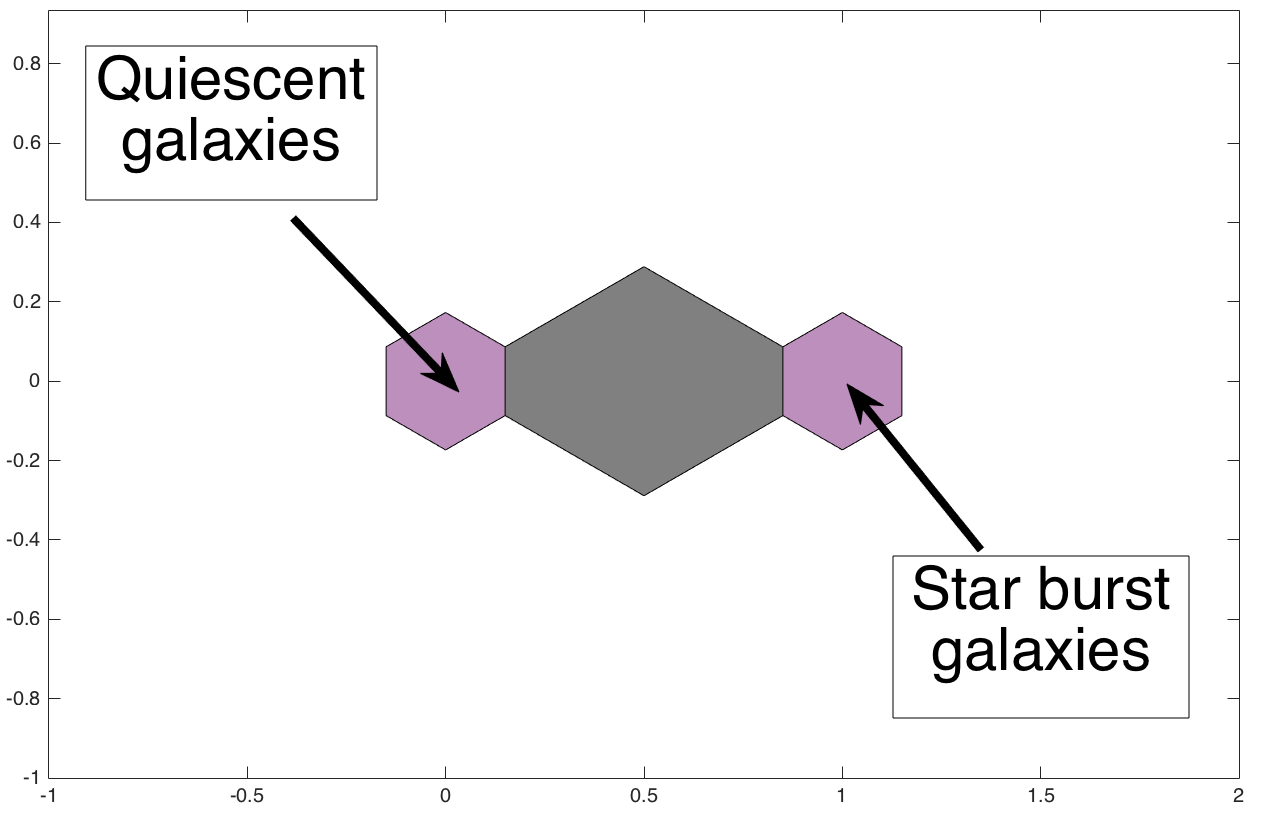
\includegraphics[width=\textwidth]{images0.01/1d/dist_1_by_2.png}
                \end{subfigure}
                \hfill
                \begin{subfigure}[b]{0.5\textwidth}
                     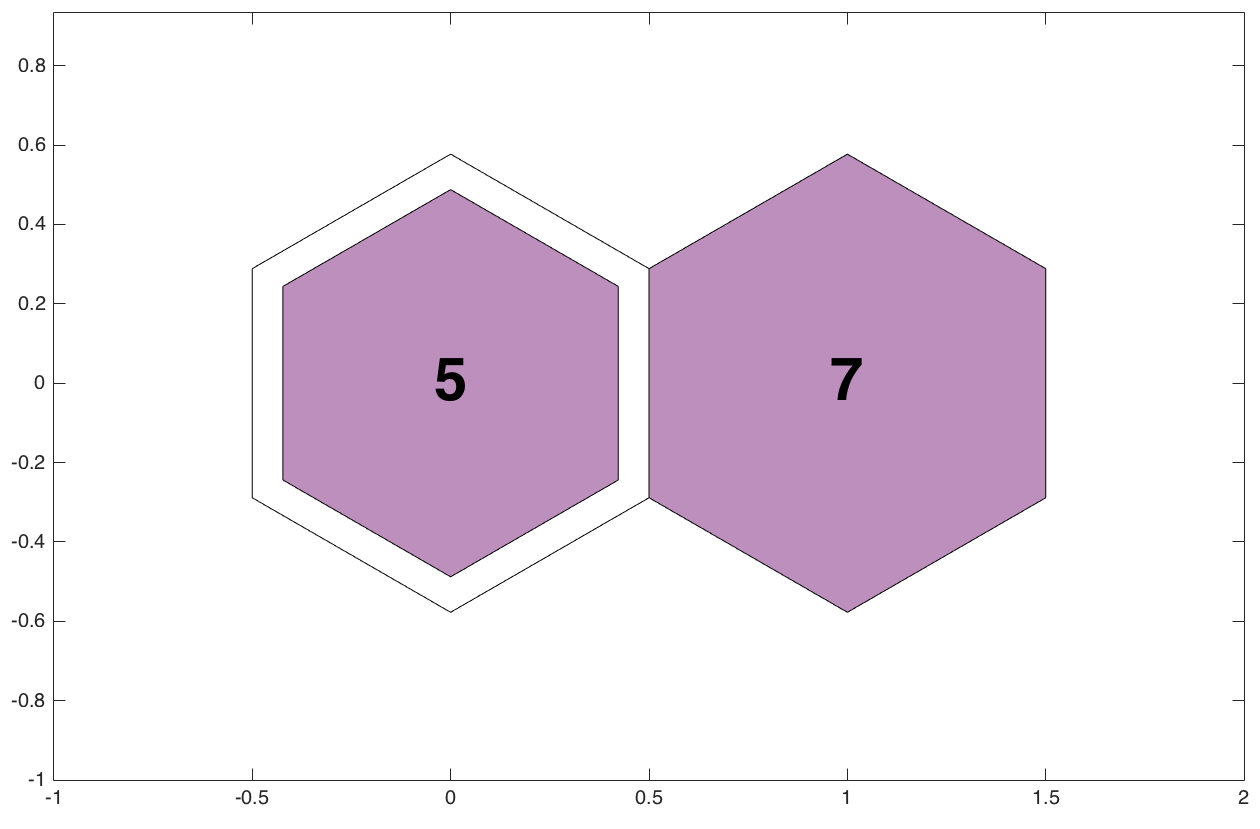
\includegraphics[width=\textwidth]{images0.01/1d/hit_t_1_by_2.png}
                \end{subfigure}
                \caption{Results of training network in $1\times2$~grid. As in Fig.~\ref{fig: sample}, the upper panel is a distance map and the lower panel is a hit map. In this network, 5 of the templates from K96 are categorized as quiescent galaxies and the rest are starbursts. Because of their strong emission lines, Sc galaxies are moved towards the starburst ones.}
                 \label{fig: 1by2T}
            \end{figure}
        
        
            In the upper map in Fig.~\ref{fig: 1by2T}, the dark colour between two neurons indicates that the relative distance between these two groups are relatively high, and these two groups are distinguishable groups.%(why do you keep reaping that?)
            In the lower part of Fig.~\ref{fig: 1by2T}, we see that the templates are divided into two groups of 5 and 7.
            Although we know from K96 and T12 that 6 of the templates are quiescent and the other 6 are starbursts, the SOM results show 5 of the galaxies in one group and the other 7 in the second group.
            In this method, the Sc template has been categorized as starburst due to the relatively higher disk stellar population relative to that of the bulge. 
            According to K96, Sc galaxies are considered to be late Hubble type galaxies which have a flattter SED compare to other quiescent galaxies. 
            

            Fig.~\ref{fig: 1by3T} shows the results of the training in a 1$\times$3 network.
            In these plots we force the galaxies to be categorize in a maximum 3 groups. 
            %If the galaxies in Fig.~\ref{fig: 1by2T} were very similar to each other or were exactly the same, they still wanted to be divided into two groups and left the middle node empty(this sentence does not make much sense. I kind of think I know what you're trying to say (because once I translate this sentence to farsi word by word, it kind of comes together) but please phrase it more carefully.).
            %[suggested sentence: 
            If the templates in Fig.~\ref{fig: 1by2T} truly belonged in two groups, they would be grouped into two groups in this network, even when we try to cluster them into three. 
            However, in the lower panel of Fig.~\ref{fig: 1by3T}, we can see that the middle node contains two templates.
            These two templates, which are separated from the group of starburst templates in the lower part of Fig.~\ref{fig: 1by2T},  are the SB5 and SB6 types.
            In the upper plot of Fig.~\ref{fig: 1by3T}, the colour between two right neurons is black and the colour between two left neurons is white. 
            The black colour indicates that the left neuron is completely different from the other two groups,
            while the white colour shows that the two right neurons are very similar to one another. 
            
            Comparing Fig.~\ref{fig: 1by2T} to Fig.~\ref{fig: 1by3T} shows that the starburst templates are divided into two groups. 
            Based on the colours between these two groups, we conclude that they are very similar; both groups are starbursting and have strong emission lines.
            On the other hand, the SB5 and SB6 templates have the highest internal extinctions; this causes the SED to become flatter at shorter wavelengths. 
            The flatter UV SED makes these two templates more similar to quiescent galaxies than to other starbursts.
            Therefore, in the networks, SB5 and SB6 types are to be grouped close to the early type galaxy templates.
                
            \begin{figure}
                \begin{subfigure}[b]{0.5\textwidth}
                    \centering
                    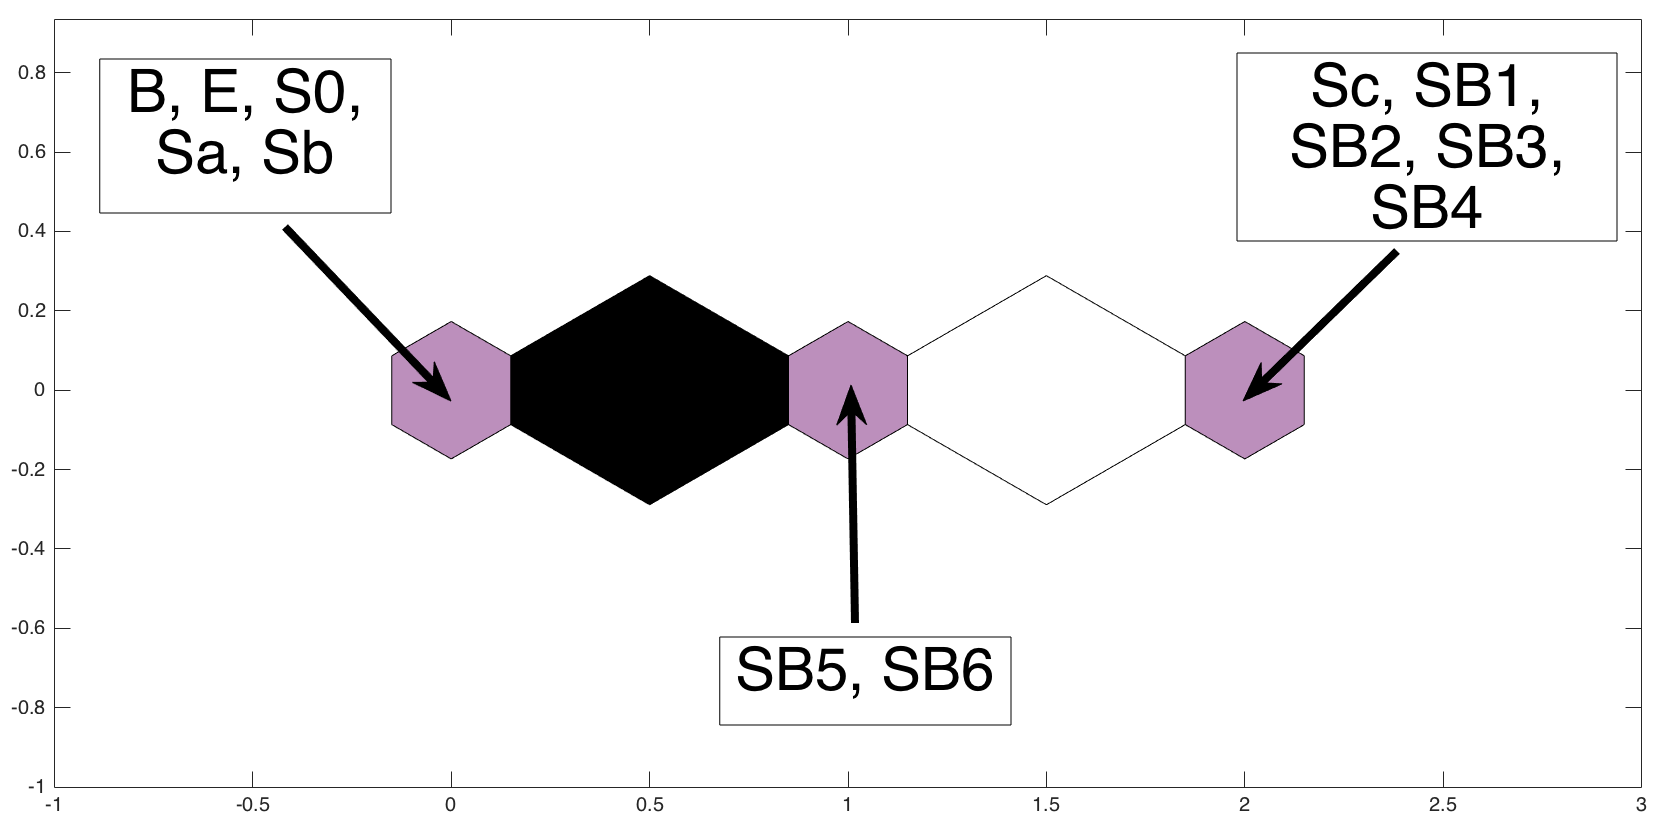
\includegraphics[width=\textwidth]{images0.01/1d/dist_1_by_3.png}
                \end{subfigure}
                \hfill
                \begin{subfigure}[b]{0.5\textwidth}
                     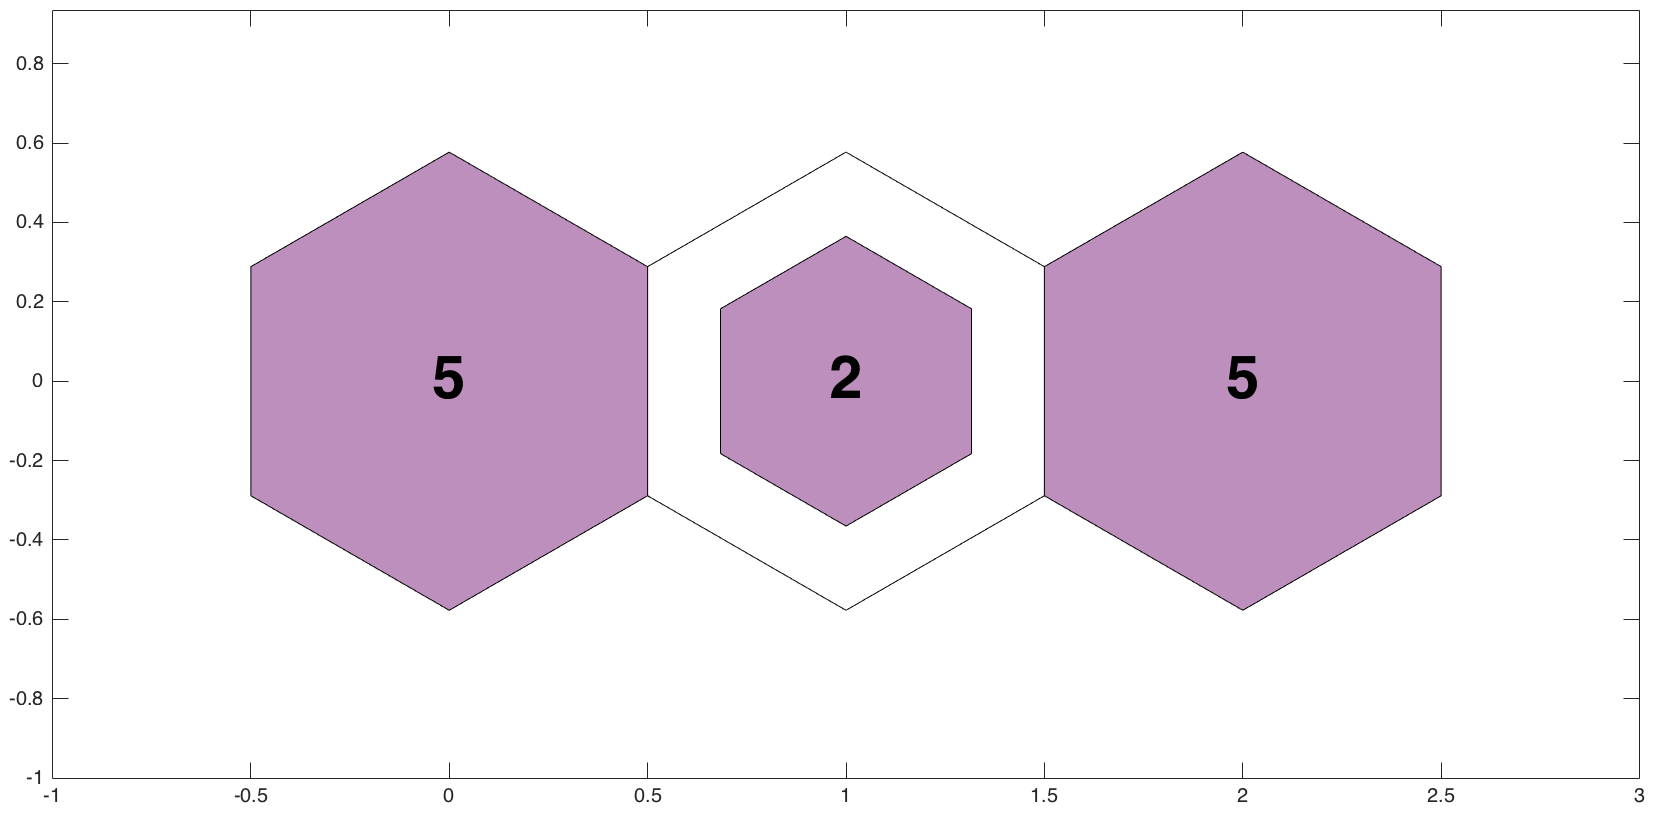
\includegraphics[width=\textwidth]{images0.01/1d/hit_t_1_by_3.png}
                \end{subfigure}
                \caption{The same as Fig.~\ref{fig: 1by2T} but showing the results of training network in $1\times3$~grid. In this network again, 5 of the K96 templates are categorized as quiescent and 7 as starbursts. However, this time 2  templates (SB5 and SB6) are separated from the starburst groups.}
                 \label{fig: 1by3T}
            \end{figure}
           
            We increased the size of the maps gradually until the galaxies are divided into twelve groups (Figs.~\ref{fig: 1by4T} to ~\ref{fig: 1by20T} and ~\ref{fig: 1by22T}).
            Since there are more nodes in higher grid SOMs, the  algorithm %program%(program? definitely use something else; like the algorithm?)  - algorithm is better - PB.
            pays more attention to small differences between groups.
 %           Increasing the size of maps means that even the smallest differences between galaxies have to be considered.
            If the templates from K96 had completely distinct SEDs, then a $1\times12$-sized SOM would be expected to show 12 different groups each containing a single template.
            However, in Fig.~\ref{fig: 1by12T}, we see that three of the neurons contain two templates and three of them are empty.
            It is evident that there was no template in the K96 sample that can fill those empty neurons.
            In Fig.~\ref{fig: 1by12T}, from left to right, templates with types B and E, SB3 and SB4, and SB1 and SB2 are the ones grouped together. 
            The SB3 and SB4 grouping breaks when we increase the size of the network to $1\times15$~(Fig.~\ref{fig: 1by15T}).
            The SB1 and SB2 templates, however, remain in the same neuron until the size of the map is increased to $1\times20$~(Fig.~\ref{fig: 1by20T}).
            The separation between templates B and E only happens when the size of the SOM exceeds $1\times22$~(Fig.~\ref{fig: 1by22T}).
        \begin{figure*}
            \begin{subfigure}[b]{\textwidth}
                \centering
                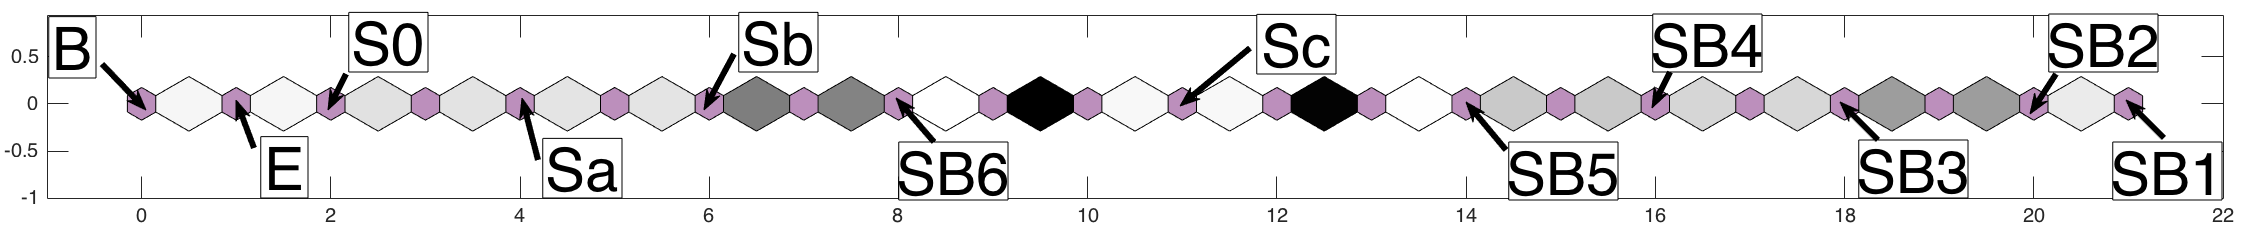
\includegraphics[width=\textwidth]{images0.01/1d/dist_1_by_22.png}
            %\caption{$1\times22$ weight map}
             %\label{fig: 1by22T}
            \end{subfigure}
            \hfill
            \begin{subfigure}[b]{\textwidth}
                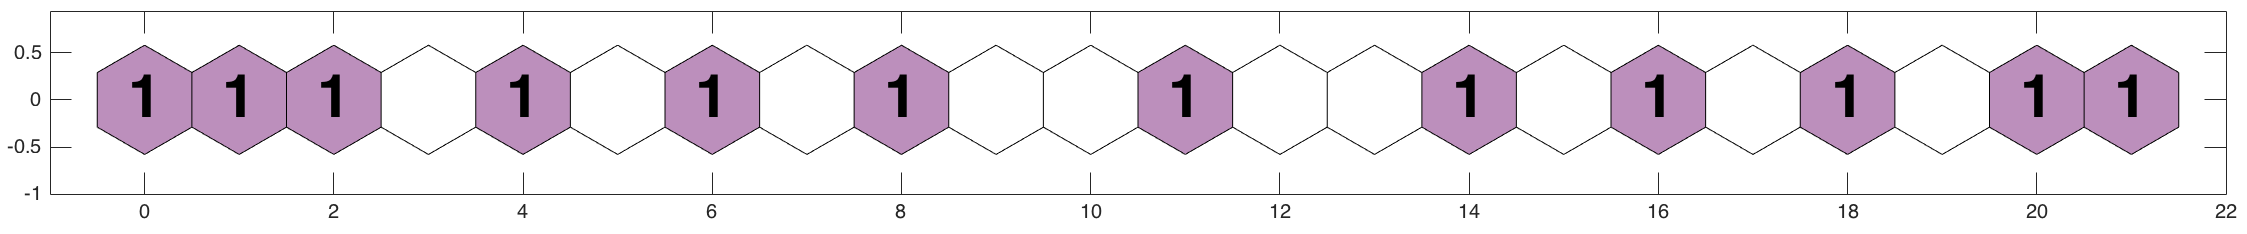
\includegraphics[width=\textwidth]{images0.01/1d/hit_t_1_by_22.png}
             %\caption{$1\times22$ hits map}
             %\label{fig: 1by22Thits}
            \end{subfigure}
            \caption{The same as Fig.~\ref{fig: 1by2T} but this time the figure shows results of training network in $1\times22$~grid.}
            \label{fig: 1by22T}
        \end{figure*} %PB160427: this figure looks really great! Very easy to understand.
    
            In Fig.~\ref{fig: 1by22T}, we can see twelve different groups:
            5 groups in the left-side neurons are separated from 7 groups on the right side of the map with two dark-grey colours between them.
            This shows that even though the galaxies are clustered in twelve groups, there still remain only two main distinct groups.
            The closest occupied neuron in the starburst side of the SOM, belongs to the SB6 type. 
            This template has the most extinction and its SED has more similarity to early type galaxies than other starburst types. 
            
            The fact that the templates need to have at least 22 different neurons to be divided into 12 groups shows that the differences between SB1 and SB2, and B and E, templates are very small.
            Because of their similarities, they tend to stay in the same group until the network becomes big enough to make attention to the smallest particularity.
           
        \subsubsection{CLASSIFYING SAMPLE OF GALAXIES}
         \label{sec: 1Dv}
            Once the networks are trained, as discussed in Sec.~\ref{sec: 1Dt}, we used them to classifying a sample 142 galaxies from T12.
            Upper plot in Fig.~\ref{fig: 1by2V} shows the result of this classification of the T12 galaxies using the $1\times2$~network from Fig.~\ref{fig: 1by2T}.
            It shows that 80 of the galaxies have SEDs similar to those of the early type galaxies and the SEDs of the rest are similar to the starburst galaxies.
            The lower plot shows the average SED of the galaxies in each node. 
            The left plot shows the average SED of 80 galaxies that were classified as an early type galaxy. 
            These galaxies are similar to the ones in the left node in the upper plot in Fig.~\ref{fig: 1by2T}.
            The plots clearly show the 4000\AA~break in the SEDs, which is one of the signatures of early type galaxies.
            The strong emission lines in the figure could be from galaxies with similar SED to Sa galaxies, but with stronger emission lines.
            The right plot in the lower part of Fig.~\ref{fig: 1by2V} shows strong emission lines and high emissions in the lower wavelengths, which are indications of high SFR in the galaxies. 
            \begin{figure}
                \begin{subfigure}[b]{0.5\textwidth}
                    \centering
                    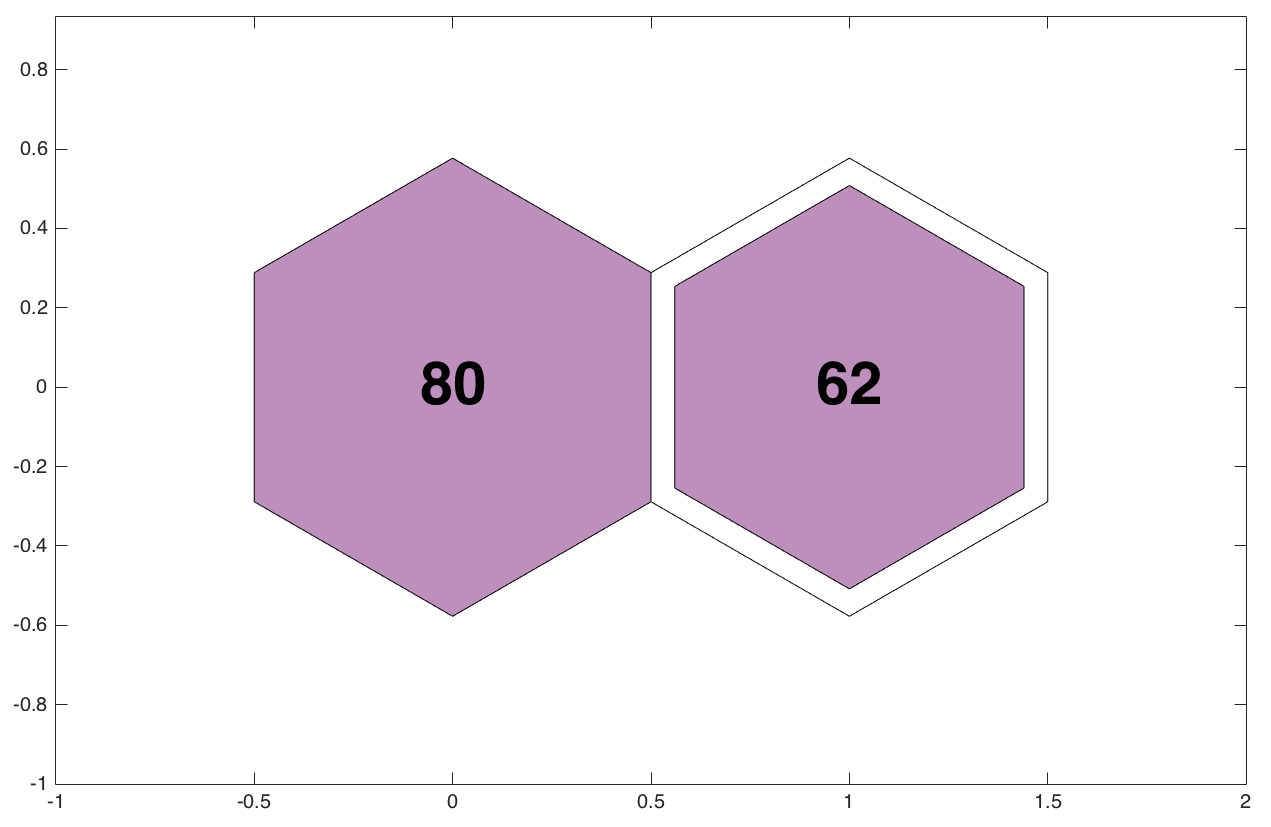
\includegraphics[width=\textwidth]{images0.01/1d/hit_v_1_by_2.png}
                    %\caption{$1\times2$ weight map}
                     %\label{fig: 1by3T}
                \end{subfigure}
                \hfill
                \begin{subfigure}[b]{0.5\textwidth}
                     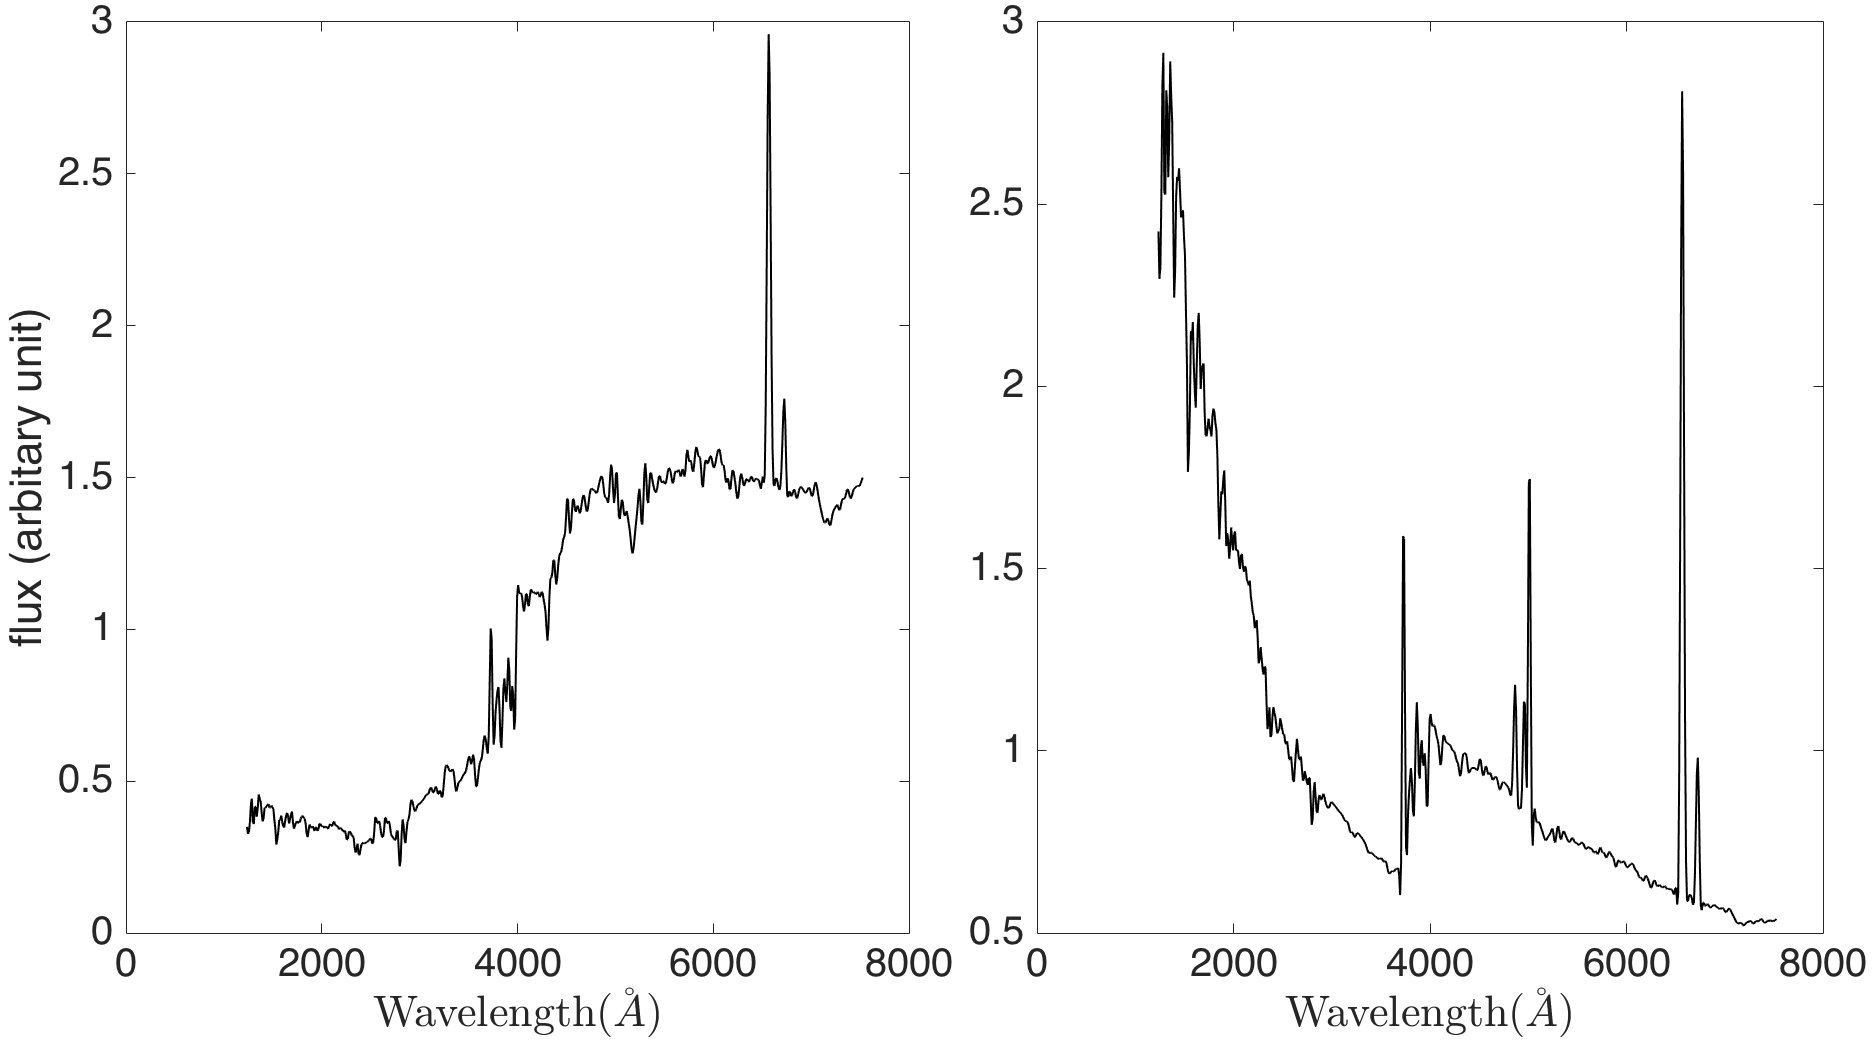
\includegraphics[width=\textwidth]{images0.01/1d/SED_total1by2.png}
                     %\caption{$1\times2$ hits map}
                     %\label{fig: 1by3Thits}
                \end{subfigure}
                \caption{Classifying galaxies from T12, based on their SEDs using $1\times2$~networks that were trained from 12 galaxies in Fig.~\ref{fig: 1by2T}. Up: the same as other hit maps, numbers in each node represents the number of galaxies that belong to that group. In this case 80 means that 80 of the 142 galaxies classify as the early type groups while the 62 of the 142 galaxies categorize to the starburst galaxies. Down: Average SED of the SEDs of the galaxies in each group. The left plot shows the average SED of the 80 galaxies (early type ones), and the right plot shows the average SED of the SEDs of 62 galaxies (the starburst ones).}
                \label{fig: 1by2V}
            \end{figure}          
            
            Since in this network galaxies were forced to be divided into a maximum of two groups, what predominantly decides which group the galaxy belongs to is the strongest feature in its SED.
            The galaxies with a weak 4000\AA~break but strong emission lines and increase of the flux in the lower wavelengths categorized as starbursts while galaxies with strong 4000\AA~break, but high emission lines categorized as the early type.
            Increasing the size of the SOM helps solve the problem of the galaxies which have features that are common in both groups.
            
            Fig.~\ref{fig: 1by3V} presents the result of classifying the SED of the galaxies using the $1\times3$~network (from Fig.~\ref{fig: 1by2T}). 
            In the upper plot of this figure we see that 66 of the galaxies belong to the early type group, and 47 belong to starburst galaxies. 
            29 of the galaxies, however, are similar to starbursts in some, but not all, of their features. 
            These groups of galaxies have strong emission lines and high flux in shorter wavelengths, but they also have a strong 4000\AA~break, which makes them cluster closer to the early type galaxies (middle plot in the lower part of Fig.~\ref{fig: 1by2V}).

            \begin{figure}
                \begin{subfigure}[b]{0.5\textwidth}
                    \centering
                    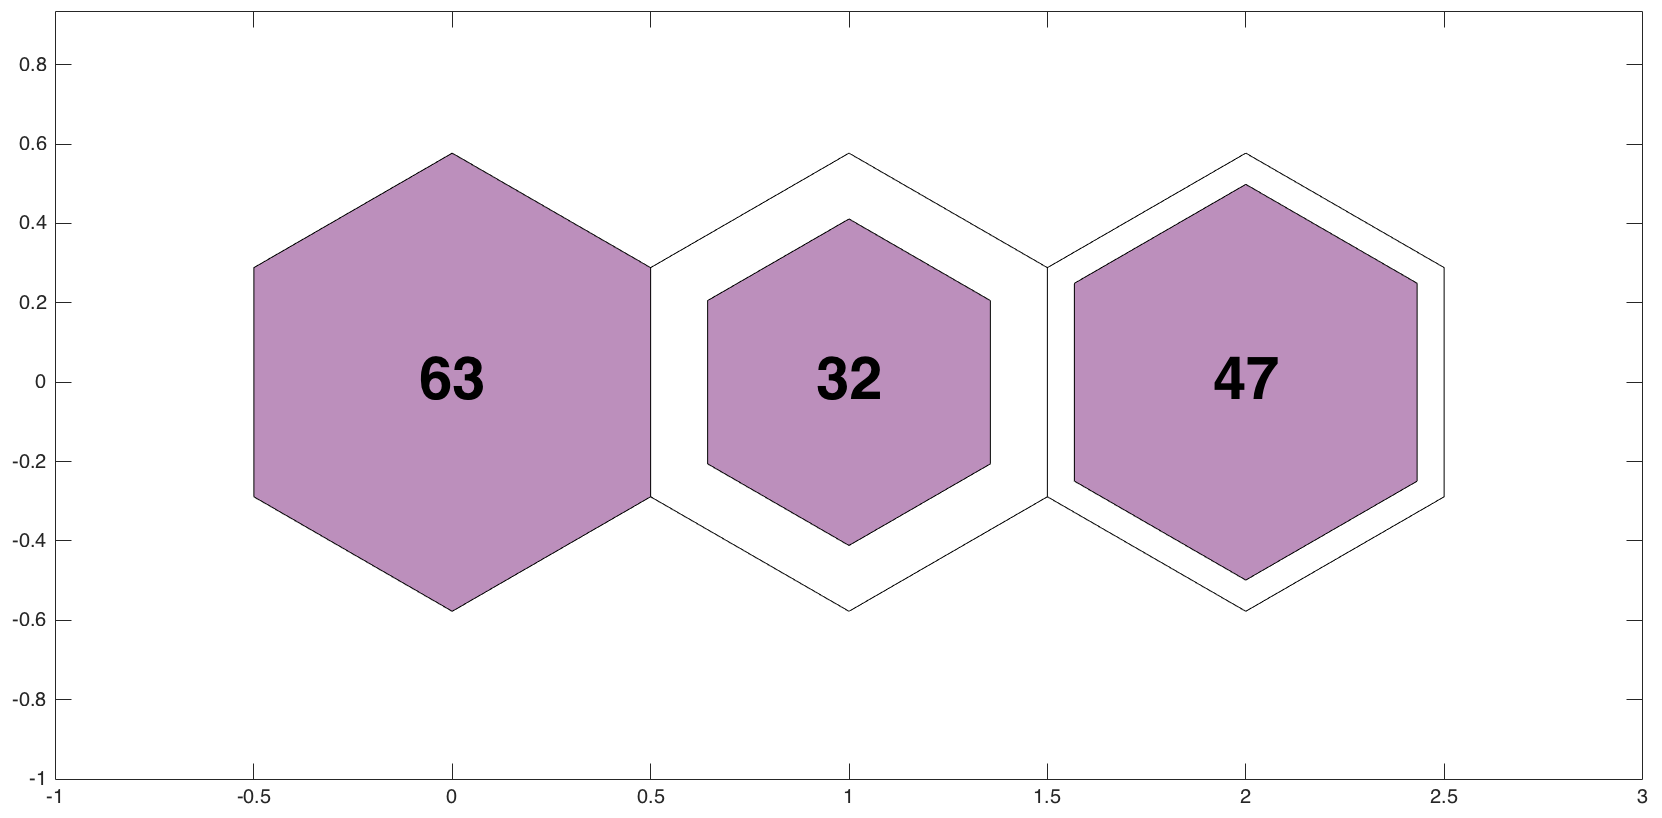
\includegraphics[width=\textwidth]{images0.01/1d/hit_v_1_by_3.png}
                    %\caption{$1\times2$ weight map}
                     %\label{fig: 1by3T}
                \end{subfigure}
                \hfill
                \begin{subfigure}[b]{0.5\textwidth}
                     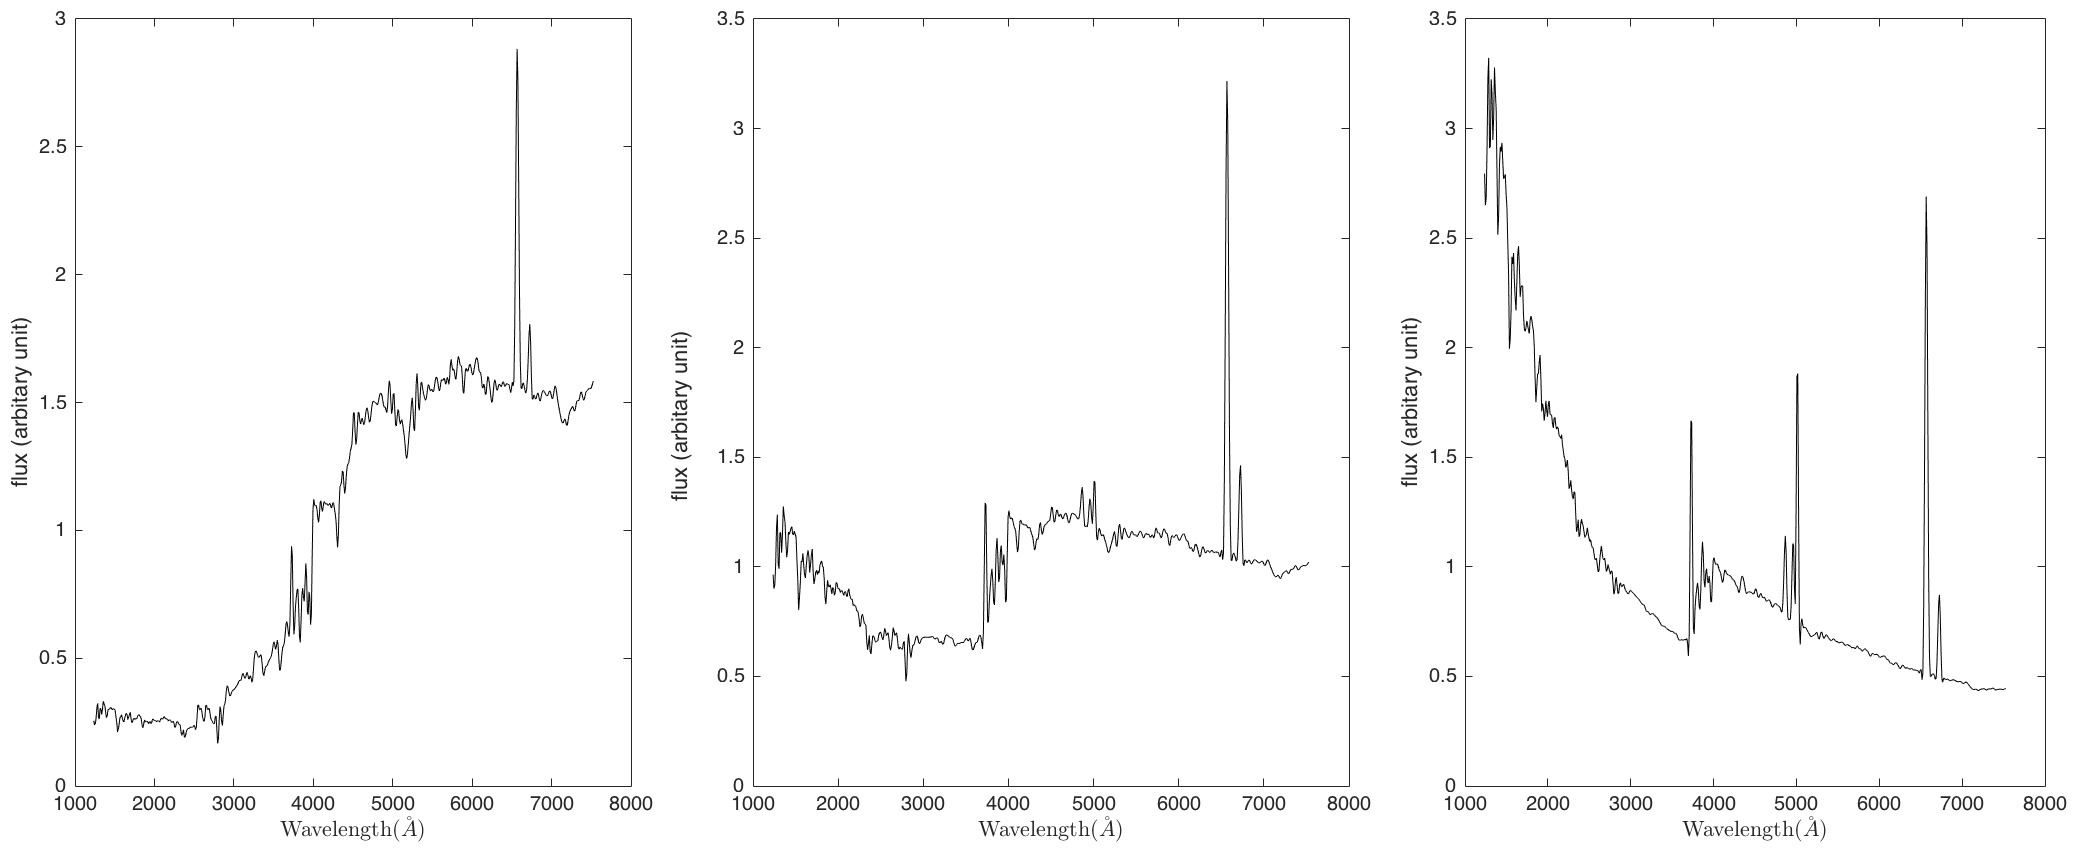
\includegraphics[width=\textwidth]{images0.01/1d/SED_total1by3.png}
                     %\caption{$1\times2$ hits map}
                     %\label{fig: 1by3Thits}
                \end{subfigure}
                \caption{Same as Fig.~\ref{fig: 1by2V}, but in this figure, we used network with size of $1\times3$ (Fig.~\ref{fig: 1by3T}) to classify the sample galaxies.}
                \label{fig: 1by3V}
            \end{figure}       
            
            In Fig.~\ref{fig: 1by22V}, we use the $1\times22$~network to classify the sample galaxies.
            As mentioned in the Sec.~\ref{sec: 1Dt}, in this network size we observed the first separation of the K96 galaxies into 12 different neurons.
            Same as Figs.~\ref{fig: 1by2V} and ~\ref{fig: 1by3V}, upper plot of Fig.~\ref{fig: 1by22V} shows the number of galaxies (out of the 142) belong in each neuron in the $1\times22$ SOM.
            \begin{figure*}
                \begin{subfigure}[b]{0.9\textwidth}
                    \centering
                    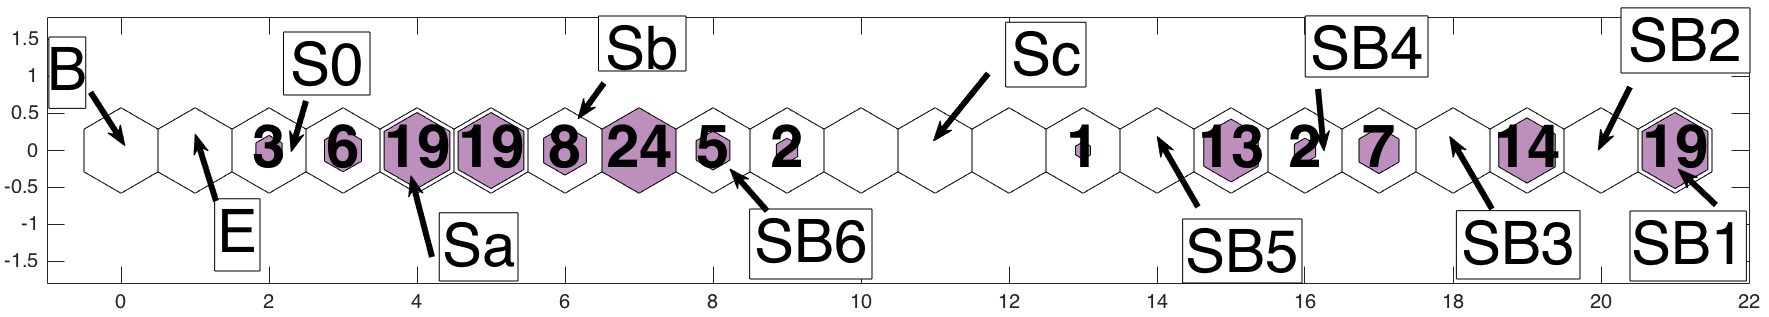
\includegraphics[width=\textwidth]{images0.01/1d/hit_v_1_by_22_n.png}
                    %\caption{$1\times2$ weight map}
                     %\label{fig: 1by3T}
                \end{subfigure}
                \hfill
                \begin{subfigure}[b]{0.9\textwidth}
                     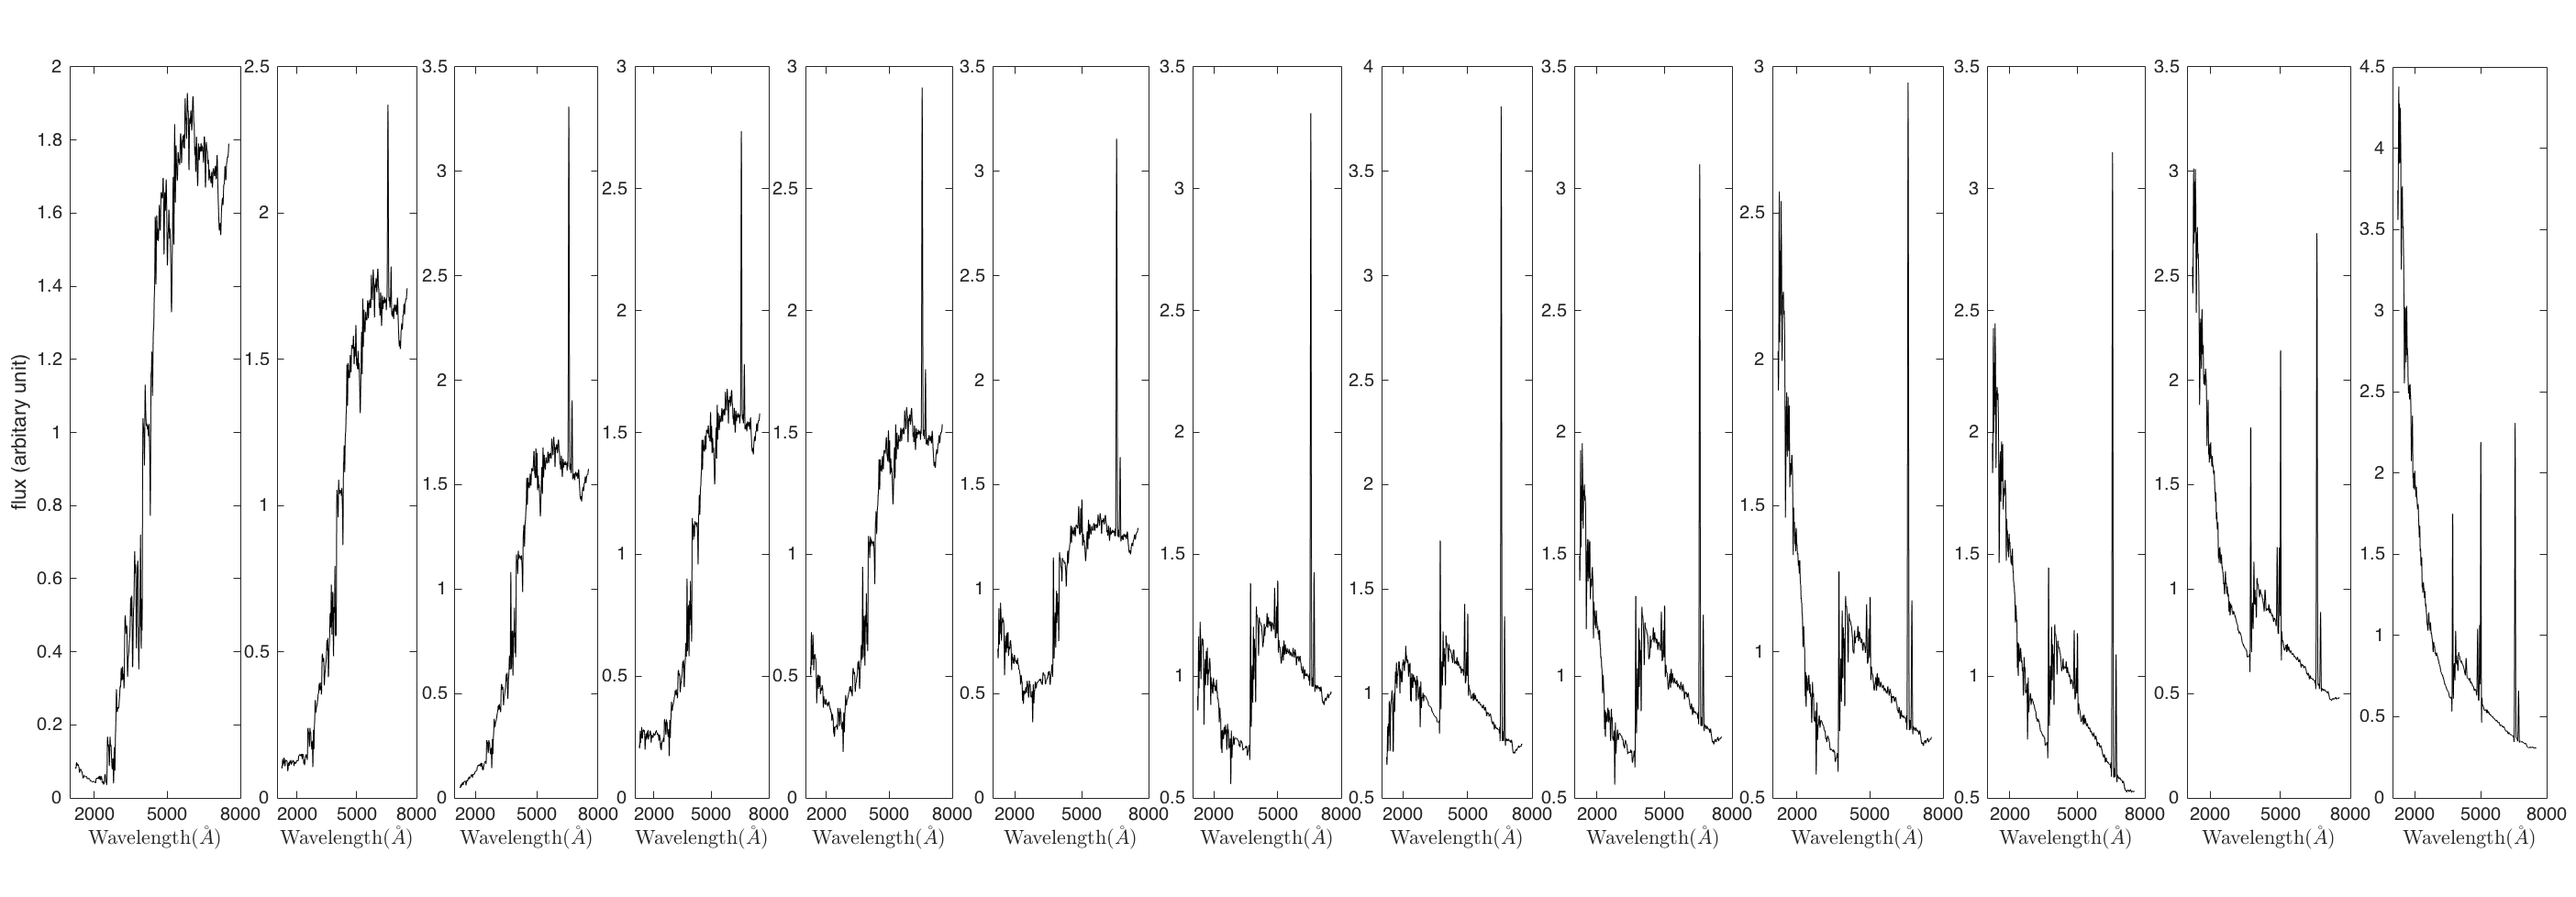
\includegraphics[width=\textwidth]{images0.01/1d/SED_total1by22.png}
                     %\caption{$1\times2$ hits map}
                     %\label{fig: 1by3Thits}
                \end{subfigure}
                \caption{Same as Fig.~\ref{fig: 1by2V}, but in this figure, we used a network with size of $1\times22$ (Fig.~\ref{fig: 1by22T}) to classify the sample galaxies. In the average SED of each neuron, we can clearly see the changes from early type galaxies in the starburst ones. 4000\AA~ break reduces from left to right and emission lines increase.}
                \label{fig: 1by22V}
            \end{figure*}
            The lower plot of the figure presents the average SED of the galaxies in each neuron.
            However, since galaxies had more space to separate, some of the neurons are left empty.
            Thus, instead of having 22 average SED plots in the lower part of Fig.~\ref{fig: 1by22V}, we only have 12.
            
            By comparing the upper part of Fig.~\ref{fig: 1by22V} with the lower part of Fig.~\ref{fig: 1by22T}, we can see that the occupied neurons are not necessarily the same.
            If a cluster from T12 galaxies fills the same neurons as the K96 galaxies ones, we can conclude that SEDs of galaxies in the cluster are very similar to those of the K96 galaxies.
            Otherwise, we can conclude that SEDs of galaxies in the cluster are similar to two of those in K96 sample.
            For the later case, the colours establish that galaxies are more similar to which ones in the K96 sample.
            
            It can be seen that the first two neurons in the upper plot in Fig.~\ref{fig: 1by22V} are empty, while these neurons were occupied by galaxies B and E in the trained network.
            We therefore conclude that there are no galaxies with specifications similar to that of the type B or E in the T12 sample.
            There are 3 galaxies in the third neuron, which shows these 3 galaxies are similar to the S0 type. 
            18 of the galaxies are on the fifth neurons and similar to the Sa type, while the 7 galaxies in the fourth neurons have SEDs similar to both S0 and Sa galaxies.
            There is one Sb type galaxy and 15 galaxies with SEDs similar to both Sa and Sb type galaxies.
            The following two neurons (eighth and ninth neurons from the left) are on the edge of the early type and starburst galaxies.
            In the upper plot in the  Fig.~\ref{fig: 1by22T}, the colour between these two neurons are black, which shows that these two are very different.
            Therefore, 24 galaxies in the eighth neurons have similar SEDs to Sb type galaxies, and SEDs of the 14 galaxies in the ninth neurons are similar to the SB6 galaxies.
            The far right neurons in the network belongs to galaxies with SED comparable to type SB1 and SB2.
            
            In general, 56 galaxies correspond exactly to K96 types and the other 86 are placed between the initial 12 suggestions.
            As T12 mentioned, part of the reason we could not classify all the galaxies using the K96 model is that the model was constructed from co-adding 12 spectra of the 70 galaxies.
            In this small sample, it is quite possible that the best SEDs do not match any model perfectly and the original classifications have high uncertainties.
            
            On the other hand, the other methods e.g. $\chi^2$ fitting, trained neural network of fitting SEDs are limited to models, and the results are always reported with uncertainties.
            However, with SOM, we have the freedom to categorize galaxies in intermediate groups.
            Therefore, if the SED of galaxies do not match completely with any of the model SEDs in Fig.~\ref{fig: k96}, they can be categorized as a SED with similarity to two or more of the groups.

                        
        
        
        \subsubsection{RESULTS PROPERTIES OF CLUSTERED GALAXIES}
        
        In order to check whether our conclusions in Sec.~\ref{sec: 1Dv}~is correct, in this section we test the relations between properties of the galaxies in each neuron.
        
        \begin{figure}
            \centering
            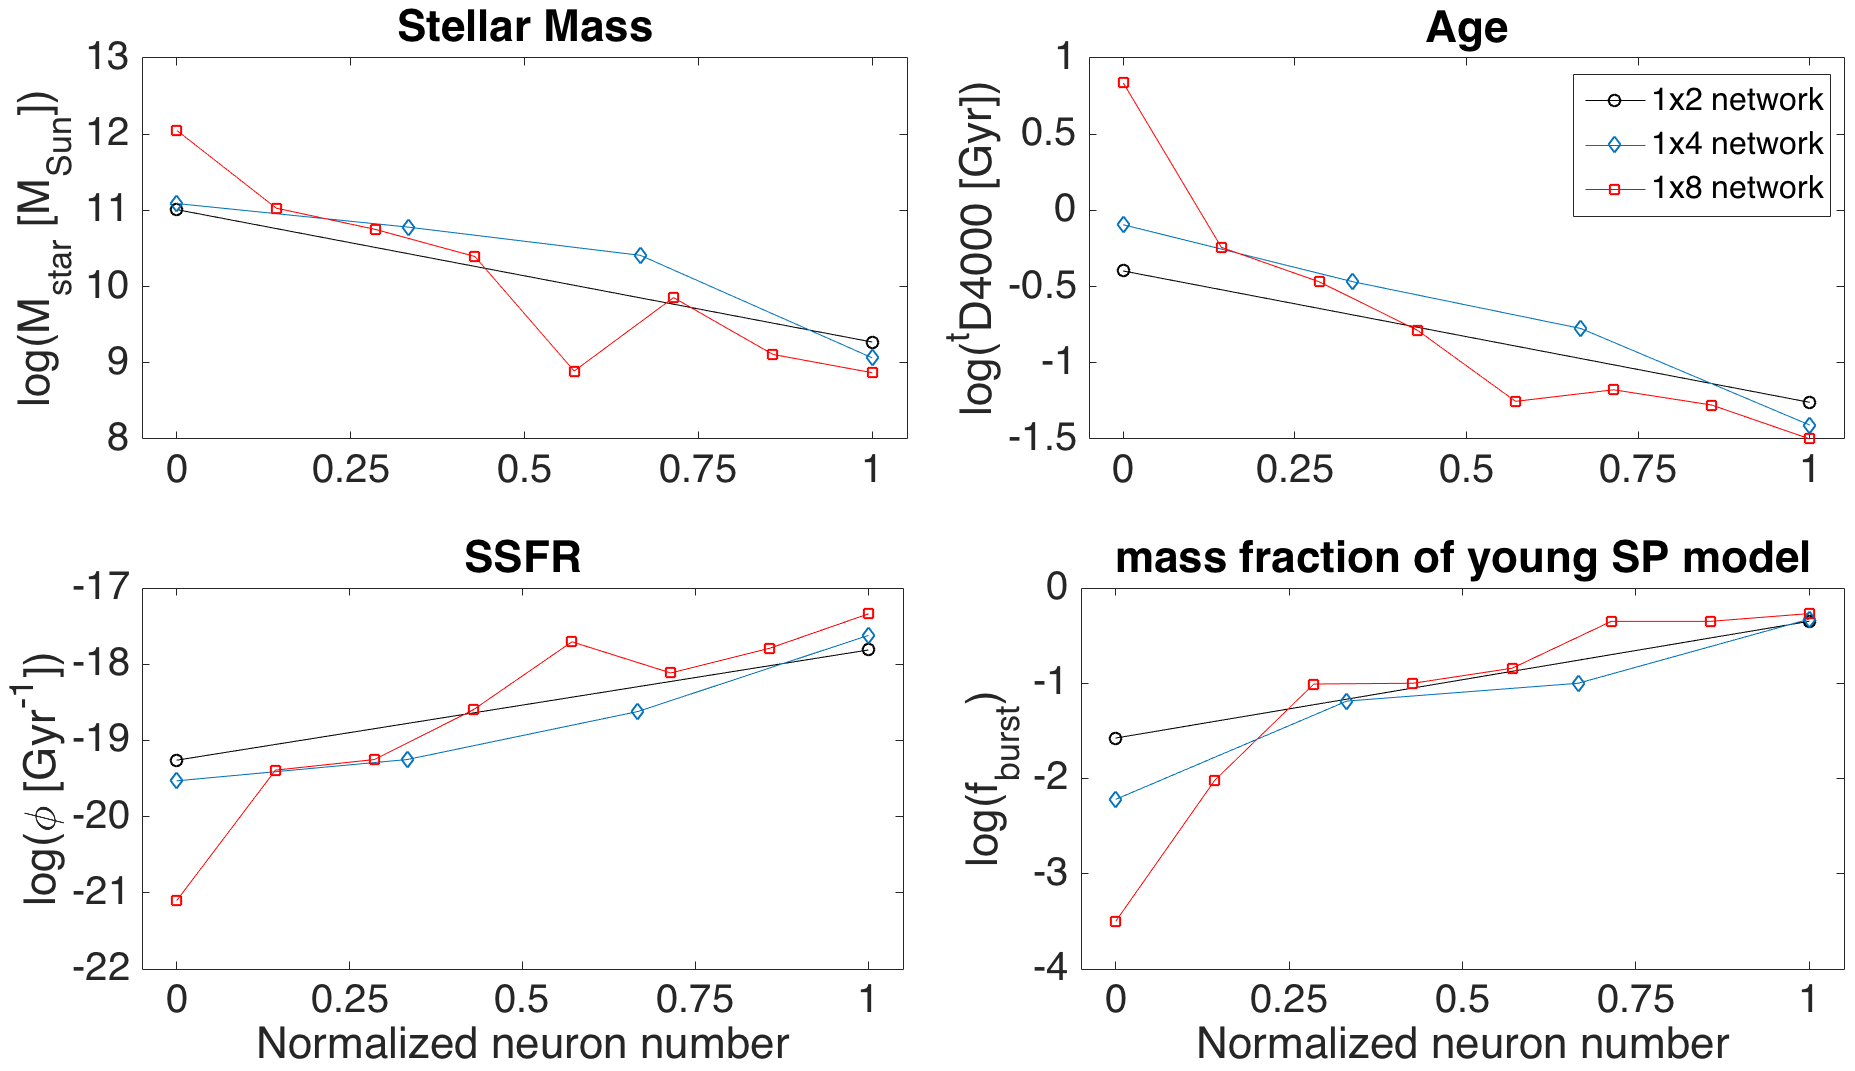
\includegraphics[width=0.5\textwidth]{images0.01/1d/props5.png}
            \caption{Comparing the median of four propertied of galaxies in each nod in $1\times2$ (balck circles), $1\times4$ (blue diamond), and $1\times8$ (red triangles) networks.}
            \label{fig: props}
        \end{figure}
       
        Fig.~\ref{fig: props} shows the results of the median of stellar mass, age, specific star formation rate (sSFR; star formation rate per stellar mass), and $f_\mathrm{burst}$ of the galaxies in each neuron in $1\times2$, $1\times4$, and $1\times8$ networks.
        In all plots, the horizontal axis is the number of the neurons divided by the size of the network, and vertical axis is one of the aforementioned properties.
        
        As shown in Fig.~\ref{fig: props}, in all three lines, stellar mass and age decrease while sSFR and $f_\mathrm{burst}$ increase as the type changes from early type galaxies to starburst ones. 
       % These trends are another evidence that this method is working and can be used to categorize galaxies based on their SEDs or even their physical properties. 
        Considering the results from Fig.~\ref{fig: props}, we can clearly see that separating galaxies based on SED types also leads to a separation in properties that derived (via {\em CIGALE}) from the SEDs.
    
        N09 used various models to derive the properties galaxies.
        Through these models, some of the properties are already known to be correlated with each others, e.g., stellar mass and star formation rate.
        They also studied other relations between properties that didn't have any direct correlation in the models in a sample of SINGS galaxies. %%eHMM I will change the previous sentence! It doesn't read well
        They found a tight correlation between sSFR and t$_{\rm {D4000}}$, which suggests that younger stellar population correlate with high SFR.
        They also found correlations between stellar mass and SFR, and stellar mass and t$_{\rm {D4000}}$.
        Since in {\em CIGALE} code, stellar mass is a free parameter, N09 argued that any stellar-mass-related correlation must be astrophysically meaningful. 
        They also studied relations between the attenuation at 1500 \AA~(A$_{\rm {FUV}}$) and sSFR, age, and stellar mass and did not find any correlation.
        T12 replicated the upper plots in Fig.~\ref{fig: props_vs_props}, and found a tighter correlation than N09 results. 
        
               \begin{figure*}
        \begin{subfigure}[b]{0.3\textwidth}
            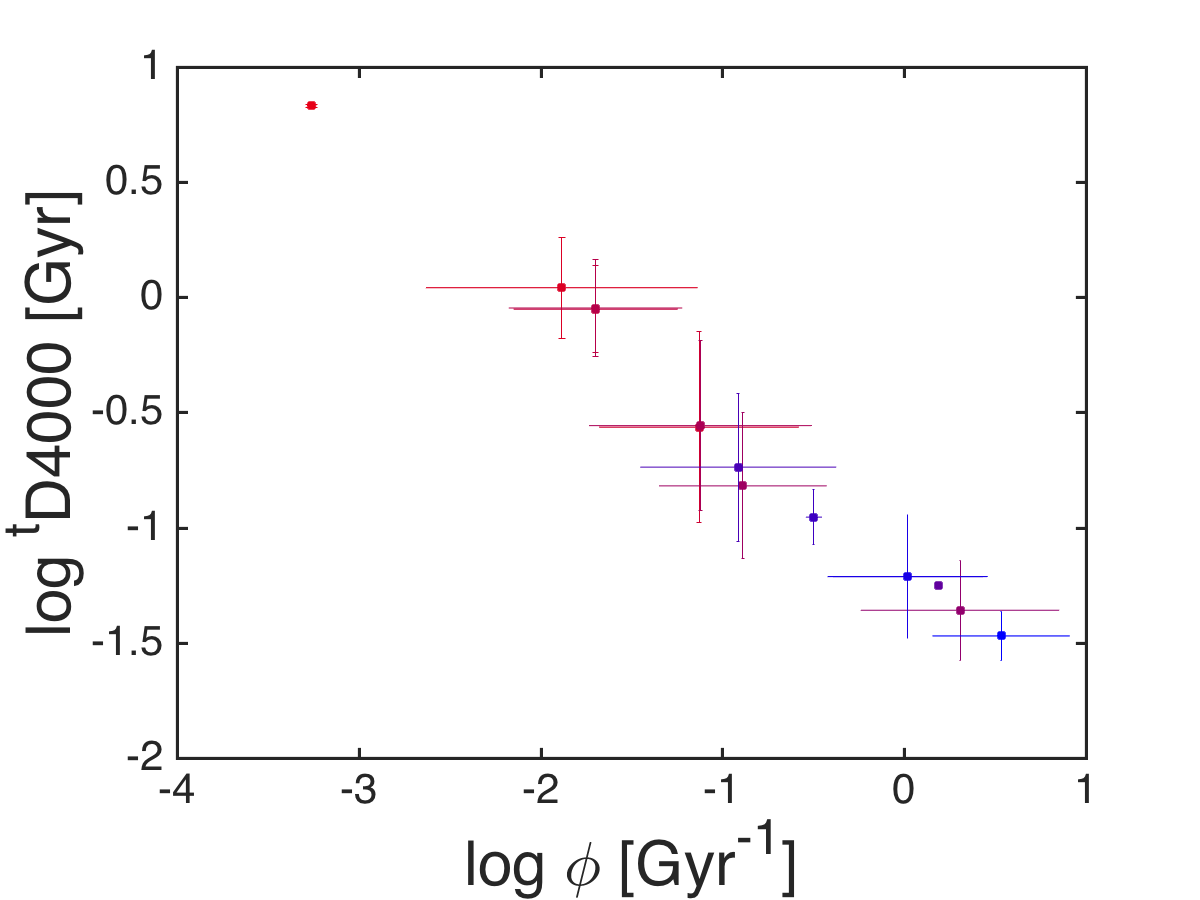
\includegraphics[width=\textwidth]{images0.01/1d/f1.png}
        \end{subfigure}
        \hfill
        \begin{subfigure}[b]{0.3\textwidth}
            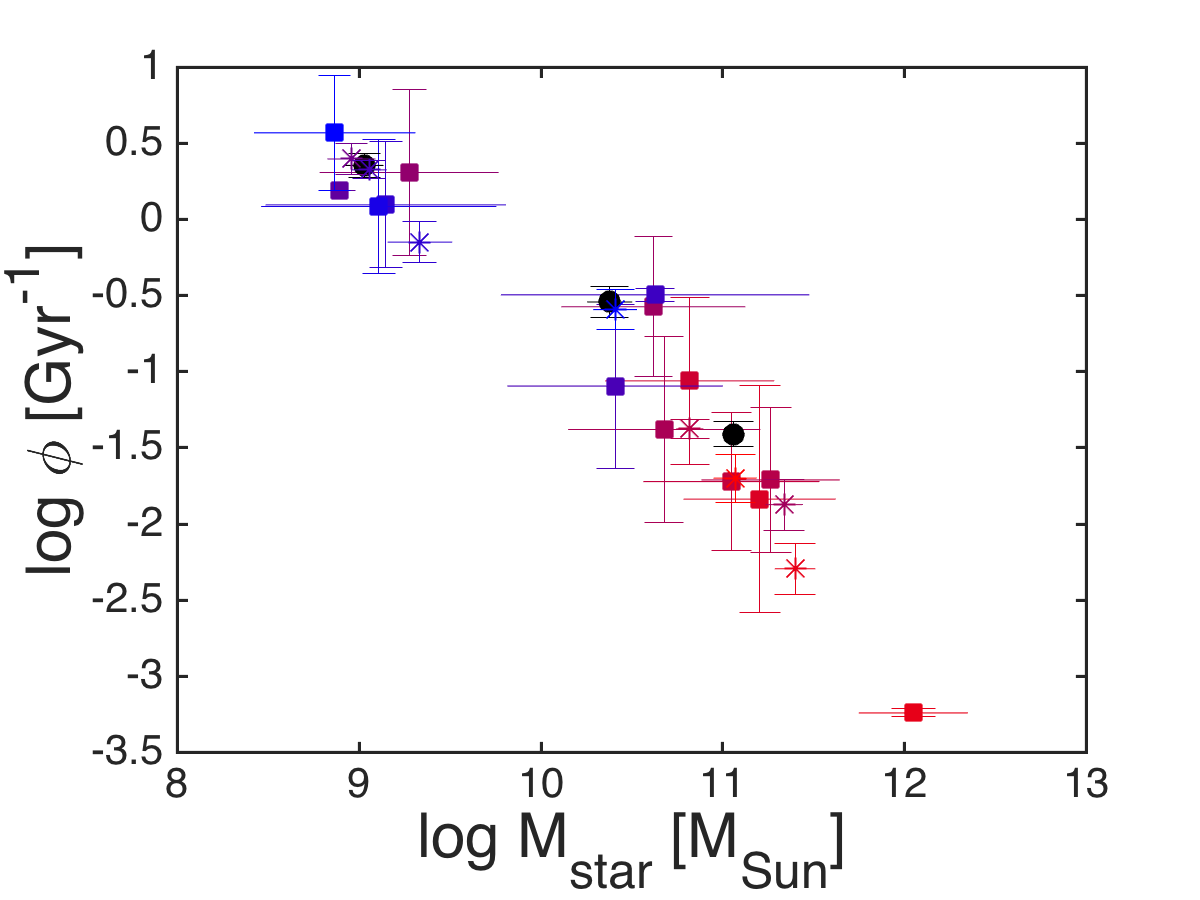
\includegraphics[width=\textwidth]{images0.01/1d/f2.png}
        \end{subfigure}
        \hfill
        \begin{subfigure}[b]{0.3\textwidth}
            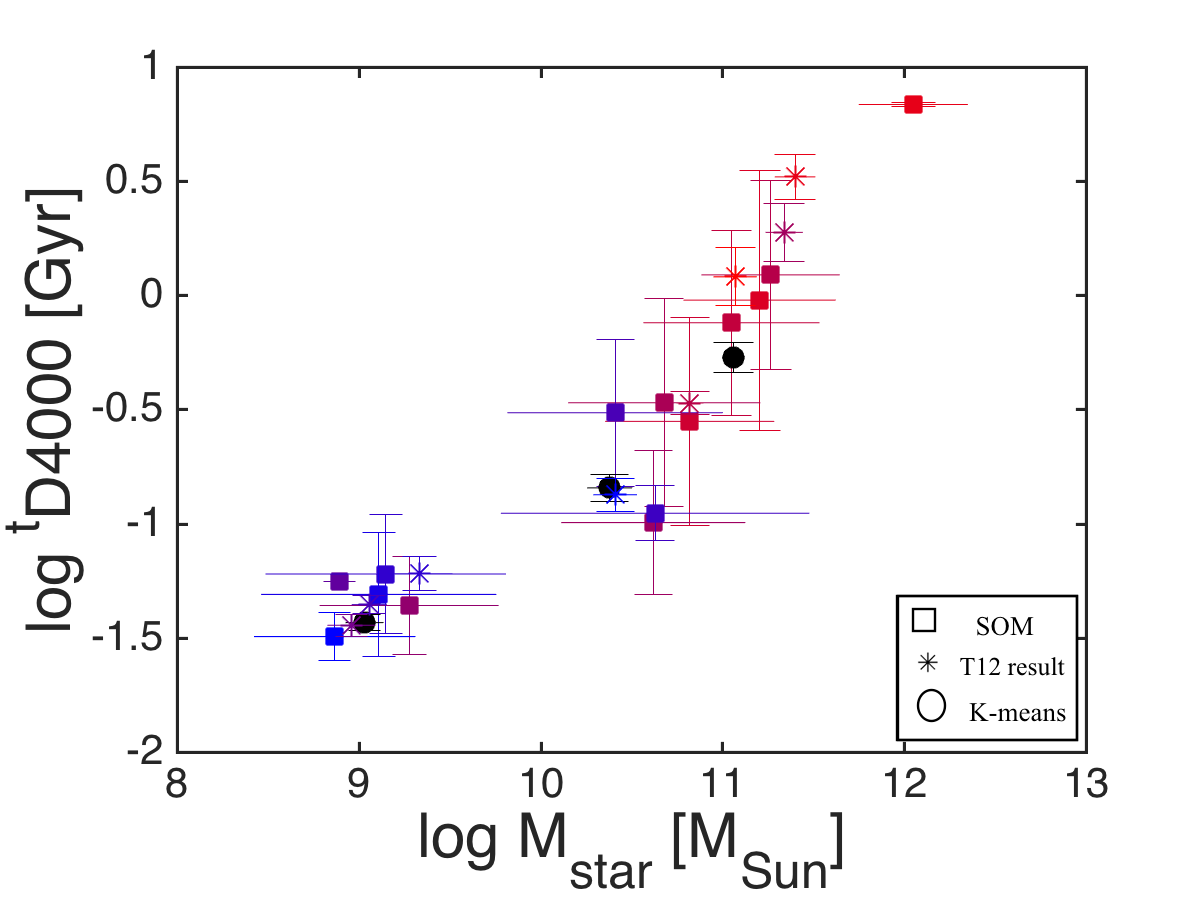
\includegraphics[width=\textwidth]{images0.01/1d/f3.png}
        \end{subfigure}
        \hfill
        \begin{subfigure}[b]{0.3\textwidth}
            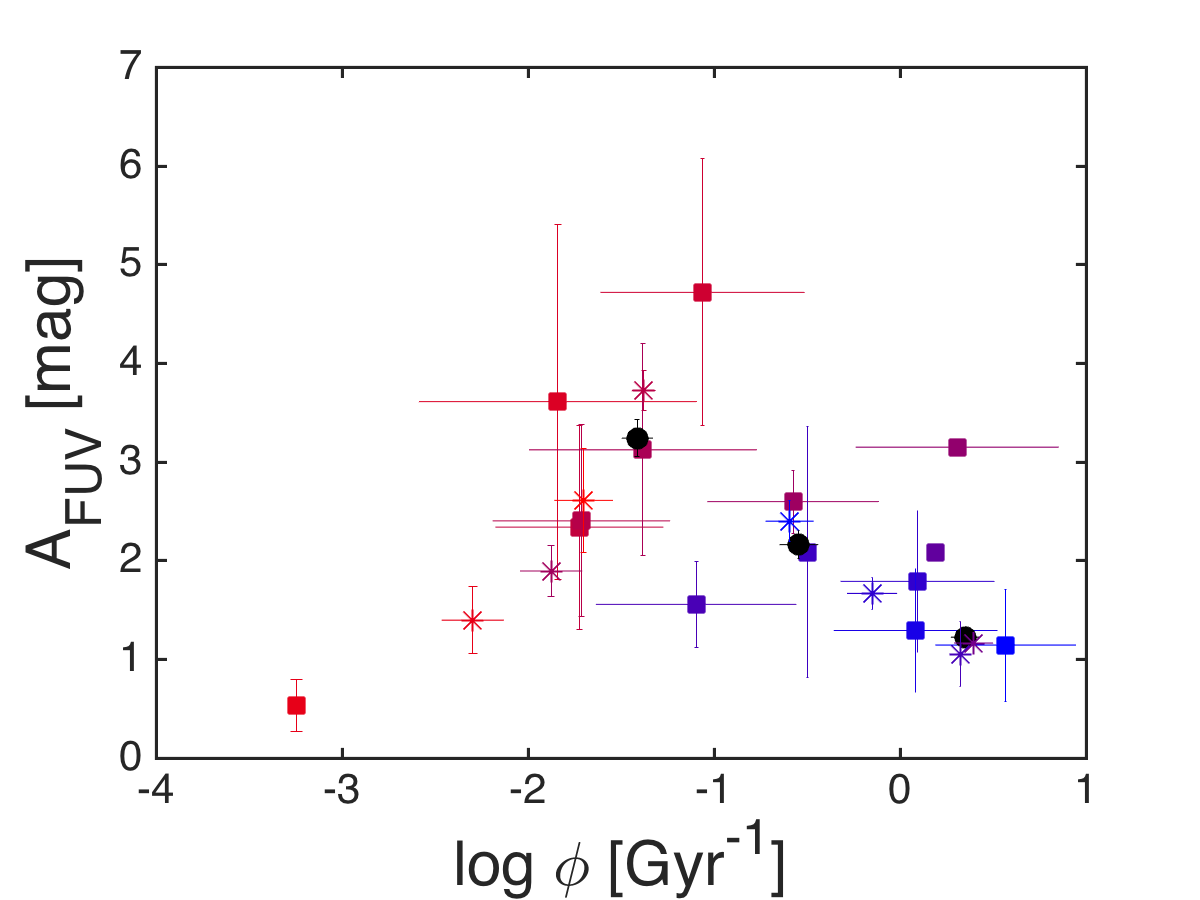
\includegraphics[width=\textwidth]{images0.01/1d/f4.png}
        \end{subfigure}
        \hfill
        \begin{subfigure}[b]{0.3\textwidth}
            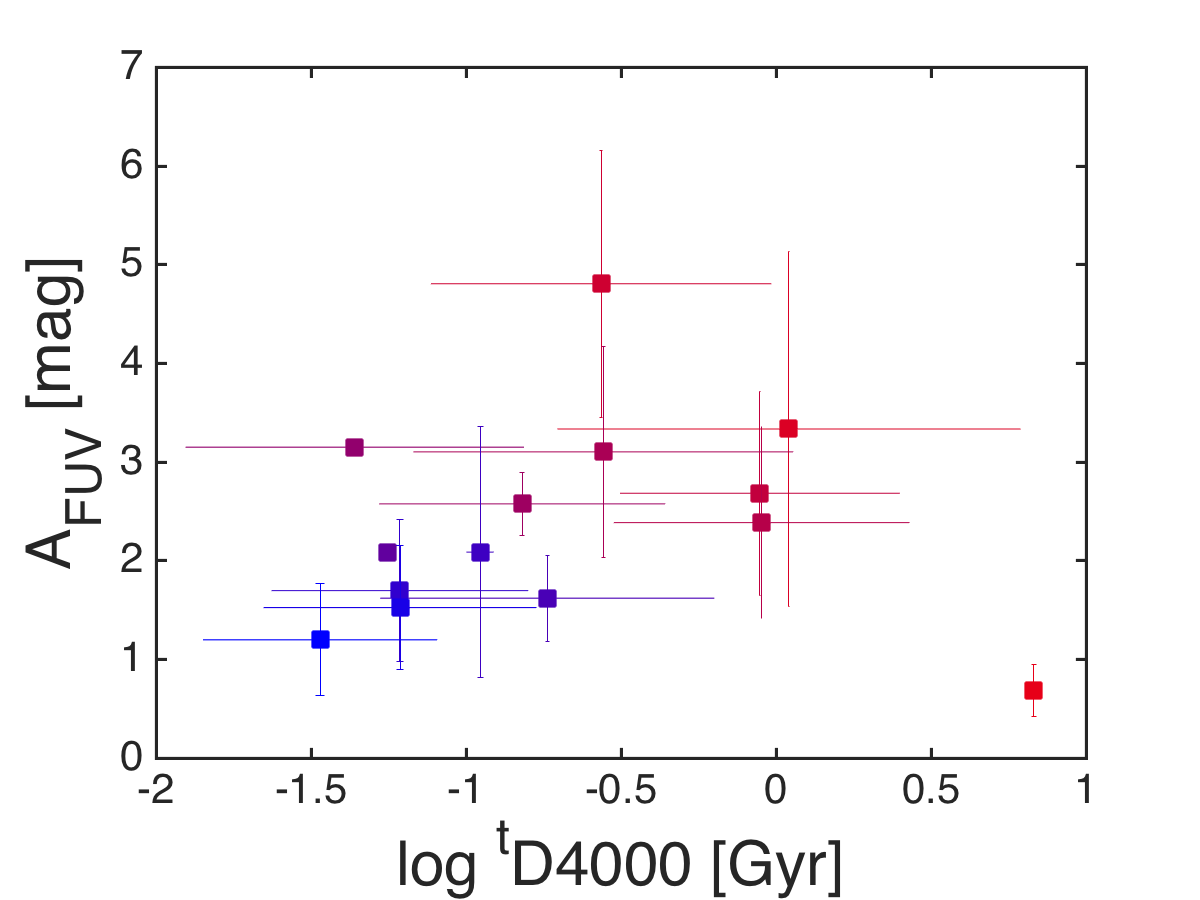
\includegraphics[width=\textwidth]{images0.01/1d/f5.png}
        \end{subfigure}
       \hfill
        \begin{subfigure}[b]{0.3\textwidth}
            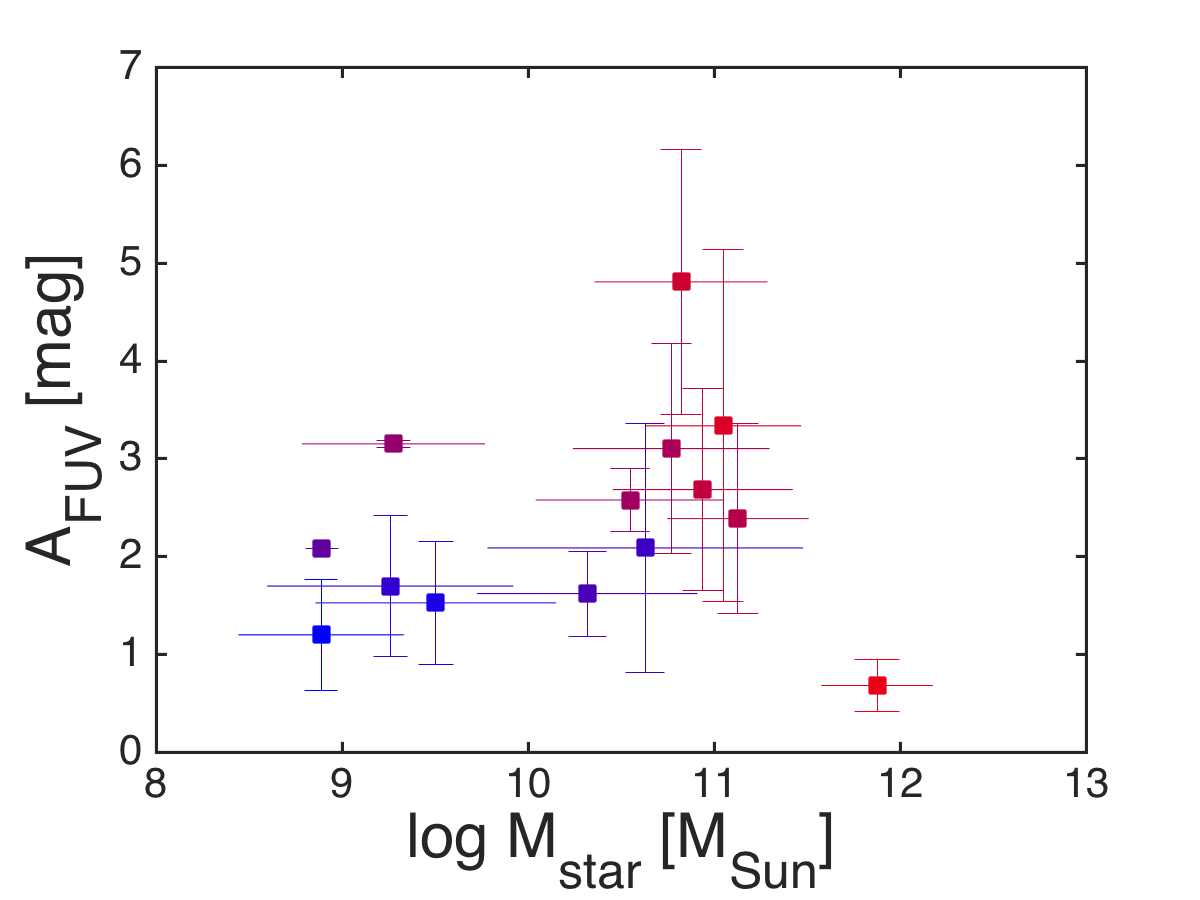
\includegraphics[width=\textwidth]{images0.01/1d/f6.png}
        \end{subfigure}
        \caption{From up to down: Correlation between age (t$_{\rm {D4000}}$) and sSFR ($\phi$), sSFR and stellar mass, age (t$_{\rm {D4000}}$) and stellar mass, and A$_{\rm {FUV}}$ with sSFR, age (t$_{\rm {D4000}}$) and stellar mass. Points show the mean values of these properties of galaxies in $1\times22$ network and error bars are the standard deviation of the mean values. colours shows the type of the galaxies in the new classification. The most pure red colour shows E type galaxies and the most blue one indicates the SB1 galaxies. The other colours depend on how much they are close to red or blue show that the galaxies are early type or starburst.}
        \label{fig: props_vs_props}
    \end{figure*}
        
        In order to compare our classifications with previous works, we produced similar plots to the ones in both N09 and T12 (Fig.~\ref{fig: props_vs_props}).
        In Fig.~\ref{fig: props_vs_props}, data points are mean values of the properties of the galaxies in each neuron in Fig.~\ref{fig: 1by22V}, and error bars show the standard deviation of those properties. 
        The colours show the galaxy types, where B type galaxies are shown with red and SB1 ones are shown with blue colours.
        The redder the colour, the more similarity with early type galaxies, while the purple to blue colours show more similarity to starburst galaxies.
        Since in this method we allow galaxies to occupy classes in between the original 12 types of the galaxies, we have more than 12 colours in Fig.~\ref{fig: props_vs_props}.
        Galaxies with SEDs more similar to type Sc having bright purple colour, but, as expected from the shape of the SED, they are old galaxies with high sSFR.
        Therefore, in all three plots of Fig.~\ref{fig: props_vs_props}, there is a purple point in the middle of the blue points.
        
        The upper plots in Fig.~\ref{fig: props_vs_props} show the same relations as N09 and T12, but with tighter correlation than those two, in all three plots.
        As mentioned in both N09 and T12, galaxies with smaller mass tend to be younger and more active.
        In Fig.~\ref{fig: props}, we see the same results: younger and more active galaxies have less stellar mass and more f$_{\rm {burst}}$.
        It is clearly noticeable that from older to younger galaxies, the colour of the points changes from red to blue, which shows a good correlation with their SED type.
        %for more details discussion on these correlations, we encourage readers to read N09 and T12.
        
        N09 studied a correlation between A$_{\rm {FUV}}$ and other properties of galaxies and showed that the attenuation has no dependency to the specific star formation, and age.
        In contrast to N09, we find a correlation between A$_{\rm {FUV}}$ and these two parameters, which are shown in lower plots in Fig.~\ref{fig: props_vs_props}.
        The general trend of the correlation that we see between A$_{\rm {FUV}}$ and sSFR in Fig.~\ref{fig: props_vs_props} is similar to the trend that have been found by \cite{Dale07}.
        They used IR luminosity to UV luminosity ratio (L$_{IR}$/L$_{FUV}$) as a measurement of A$_{\rm {FUV}}$ and compared it with sSFR for all 75 galaxies in the SINGS survey.
        They found that for early type galaxies L$_{IR}$/L$_{FUV}$ (or A$_{\rm {FUV}}$ ) correlates with sSFR, and in case of spiral galaxies, there is an anticorrelation between L$_{IR}$/L$_{FUV}$ and sSFR.
        It should be noted that, by early type galaxies they mostly meant E and S0 and S0/a types of galaxies.
        Since in our sample we do not have E type galaxies, we cannot show confidently that we see the same correlation between A$_{\rm {FUV}}$ and sSFR in early type galaxies. 
        However, it is clear in Fig.~\ref{fig: props_vs_props} that A$_{\rm {FUV}}$ increases with increasing the sSFR in the S0 and Sa types.
        The correlation in the other types of galaxies is very similar to the one that had been shown in \cite{Dale07}.
        Both \cite{Dale07} and N09 have argued that these apparent trends can be a result of the dependence of star formation history to L$_{IR}$/L$_{FUV}$.
        Whether these dependency is real or not, in this paper we showed that using SOM we can separate SEDs of galaxies on the way that the characteristic of each of these groups are in agreement with the general picture of the galaxy evolution.
        
        
    \subsection{2D SOMs}
    \label{sec: 2D}
    The 1D networks are great tools to categorize the SEDs and monitor the changes of properties of galaxies in each category.
    However, each neuron in these networks is limited to be connected to one other neuron in each direction.
    In 2D network, each neuron can have more than two immediate neighbours, therefore, they provide more complete pictures of relations between each SED type.
    As described in the Sec.~\ref{sec: method}, one of the main advantages of the SOM is that when the weight of one neuron is adjusted after finding the best matching unit, the weight of the whole map will be changed.
    This quality of the SOMs provides a unique opportunity to analyse 2D networks in two approaches. 
    At first, as we had in the 1D SOMs, we assumed that all the galaxies must have SEDs similar to any of the 12 templates in Fig.~\ref{fig: k96}.
    In this case, we can categorize SEDs of other galaxies based on those 12 types.
    
    In the second approach, we trained networks with an assumption of there might be some completely different types of galaxies that we never encountered before.
    This approach can be used to trace and recognize the outliers.
    To be able to execute the second approach, we used {\tiny selforgmap} library in {\tiny MATLAB}.
    Using {\tiny selforgmap} code, based on the size of a map and the ordering step neighbourhood distance, we can arrange that the data spread all over the SOM or sit close together.
    The latter case, can be used to identify outliers. 

    For getting the best result from both of these ways, we should have SOMs with ``high enough"  neurons to give any new sets of galaxies a chance to find their place in the map.
    The  ``high enough  neurons" is a vague statement, but as mentioned in the Sec.~\ref{sec: method} the size of SOMs is arbitrary and depends on the size of the input data and the kind of information you need from the SOMs. %PB160427: this is a feature of clustering methods in general. Maybe in the methods section where you talk about the size of maps, you could give some examples of what "what kind of information" might mean.
    Since the training data (K96 ones) have 12 galaxies, we assumed a SOM with size of $8\times8$~would be a good start.
    We then increased the size of the SOM to find the highest size suitable for the training sample.
    We noticed that SOMs with size of $12\times12$~are the maximum possible choice.
    That is increasing from $12\times12$~neurons, would not change the SOMs by much.
    
    \begin{figure*}
        \begin{subfigure}[b]{0.45\textwidth}
            \centering
            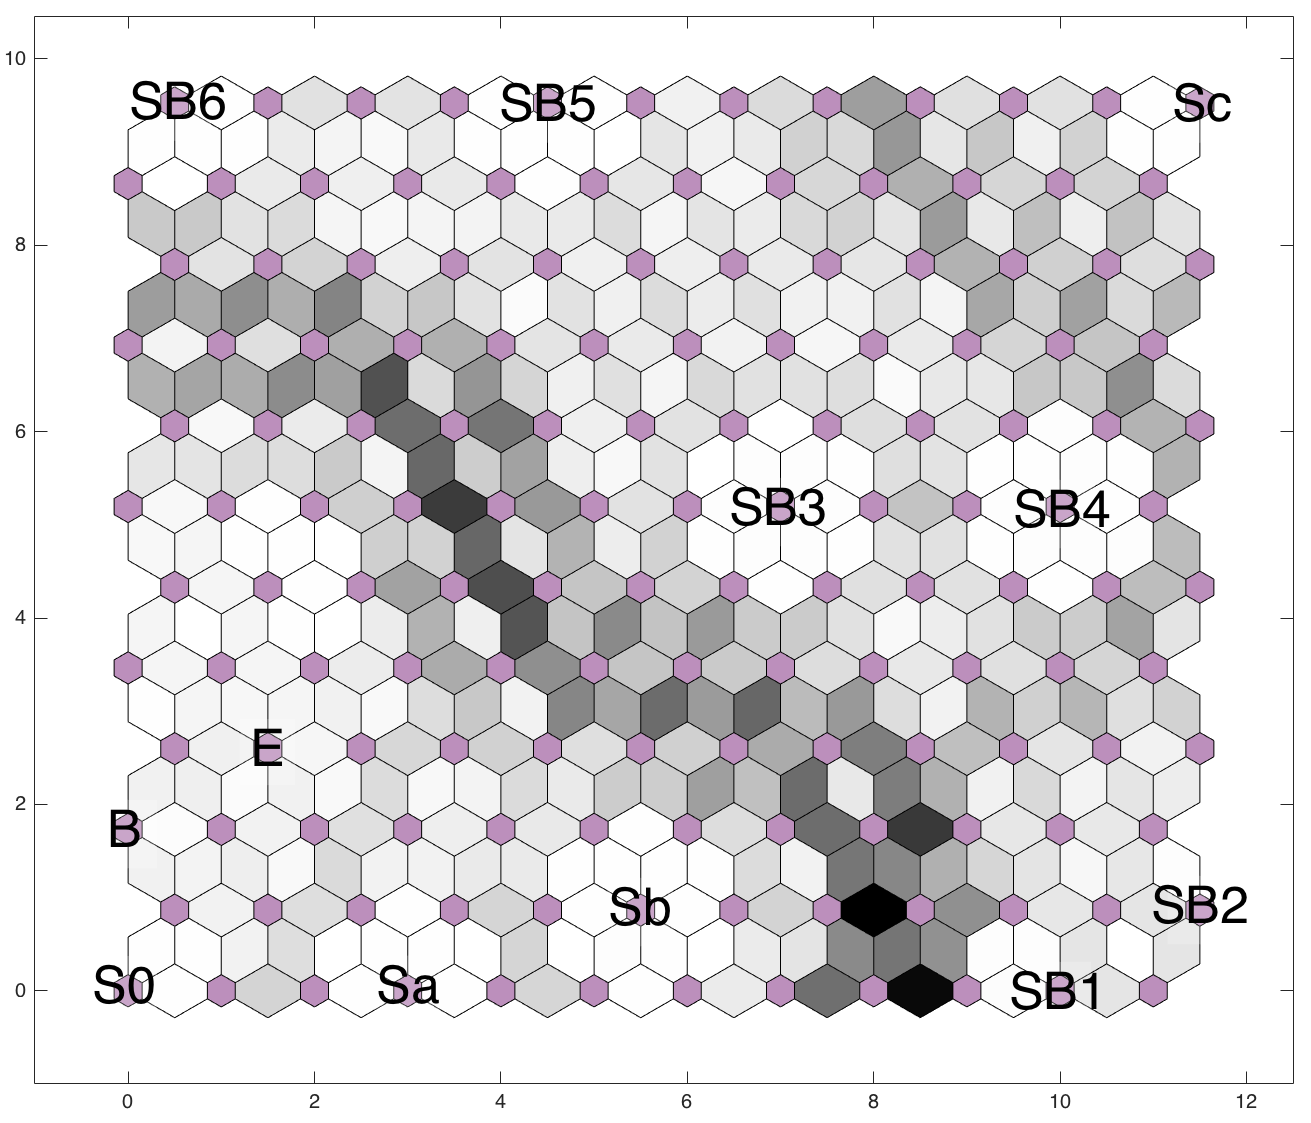
\includegraphics[width=\textwidth]{images0.01/2d/dist_12_by_12.png}
        \end{subfigure}
        \hfill
        \begin{subfigure}[b]{0.45\textwidth}
            \centering
            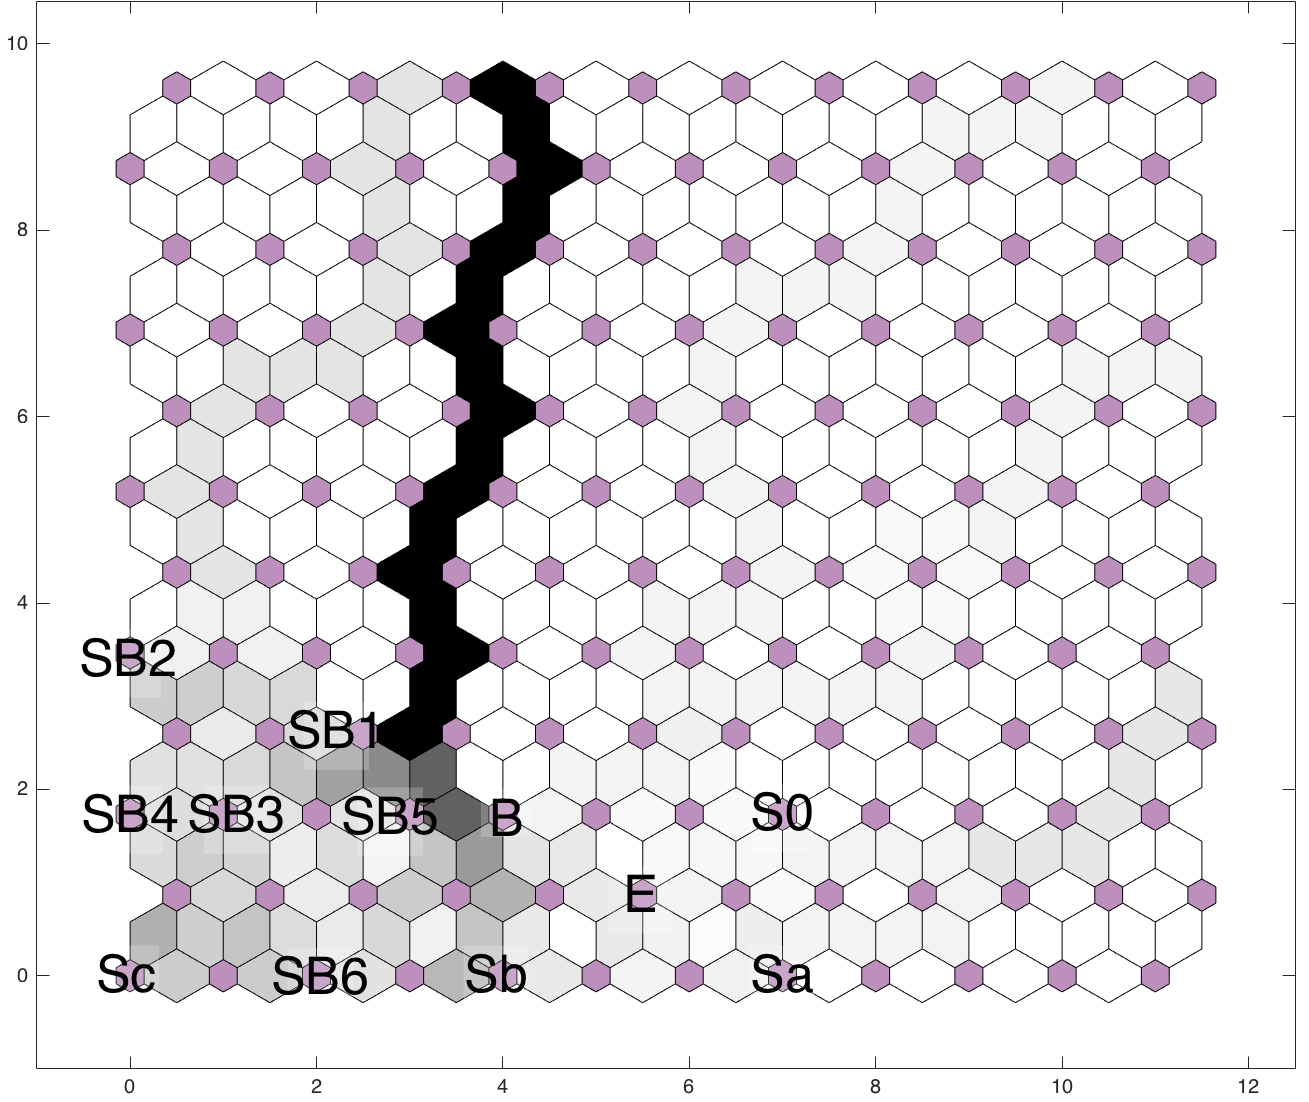
\includegraphics[width=\textwidth]{images0.01/2d/dist_12_by_self_org_res12.png}
        \end{subfigure}
        \hfill
        \begin{subfigure}[b]{0.45\textwidth}
            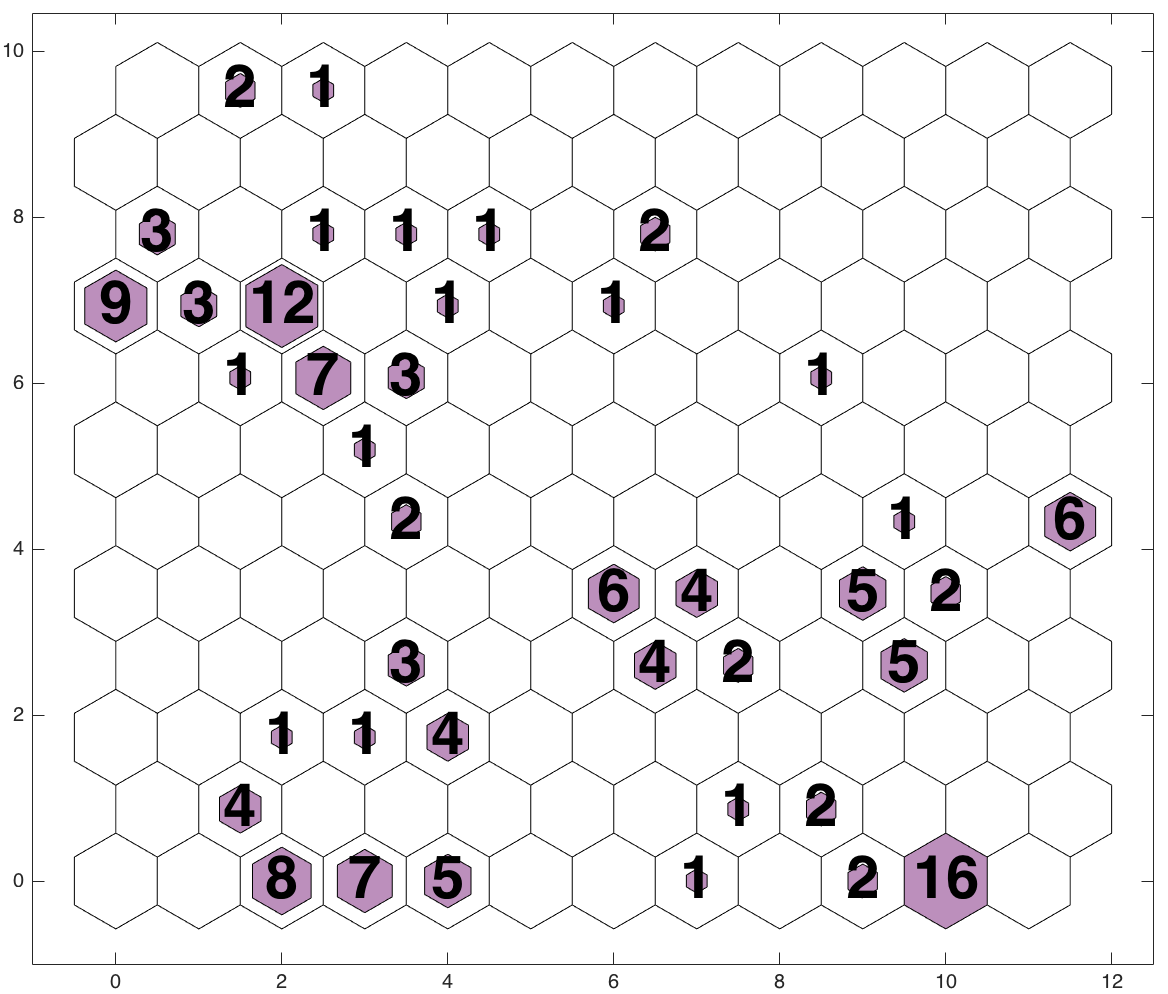
\includegraphics[width=\textwidth]{images0.01/2d/hit_v_12_by_12.png}
        \end{subfigure}
        \hfill
        \begin{subfigure}[b]{0.45\textwidth}
            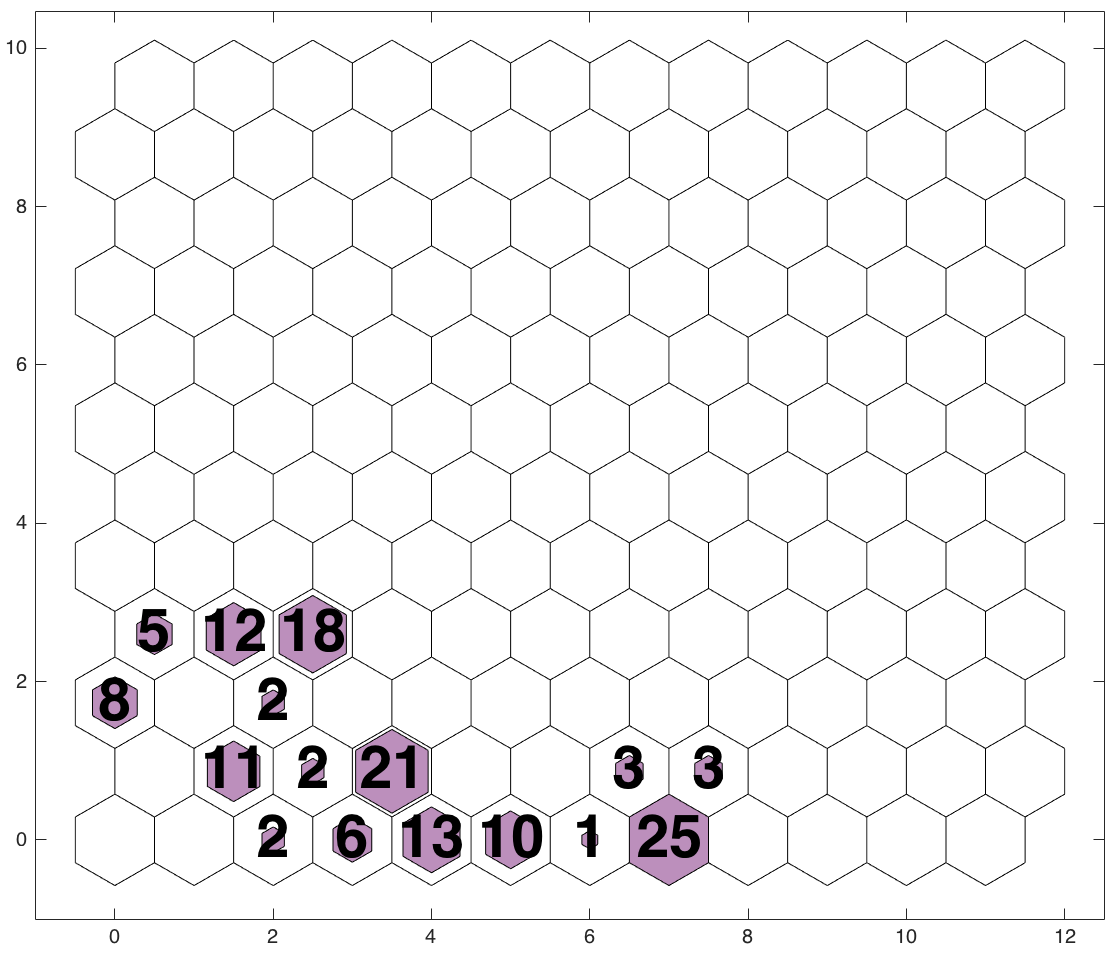
\includegraphics[width=\textwidth]{images0.01/2d/hit_v_12_by_self_org_res12.png}
        \end{subfigure}
        \caption{$12\times12$~2D SOM results. Up: Trained SOMs using K96. For training 2D SOMs two different approaches were considered; Either only 12 types of galaxies are existed (left) or not (right). Down: classifying the galaxies from T12, using the trained networks above them. From the right side one, we can see that there is no outlier in the galaxies from T12, and we can use the left side map as a final clustering results for the T12 galaxies.}
        \label{fig: 12by12}
    \end{figure*}
    
    The upper left part of Fig.~\ref{fig: 12by12} shows the SOM results from the first approach. 
    Since we considered that SEDs of all galaxies can be categorized using the K96 model, the galaxies took place all over the map.
    Using this network to categorize any set of SEDs forced the SEDs to be in the same neurons as the K96 ones or the neurons between them.
    However, all K96 galaxies are in a small side in the upper right map in Fig.~\ref{fig: 12by12}, which provide enough freedom for SED of the galaxies to take place everywhere in the map even if it is way far away from the K96 templates.
    
    
    In the upper left part of the map in Fig.~\ref{fig: 12by12}, although galaxies have more ways to be separated, they were separated in two main groups.
    There is a distinguishable strip of the grey, dark grey and in some cases black colour in the map.
    This strip is separating early type galaxies with starburst ones.
    The lower map shows that 5 of the neurons on the left side of the strip are full. 
    These five neurons are the same as the ones on the left hand side of Fig.~\ref{fig: 1by2T} (early type galaxies).
    The only difference is that here, in this map they have more space to be separated from each other.
    When we use this network to categorize the SED of galaxies, any galaxy places on the left hand side of the strip is an early type galaxy and any one placed on the right side of the strip is a starburst one.
    The decision about what type of early type or starburst galaxy, is based upon its relative position to each type in the SOM.
    
    Same as ther other map, in the upper right map in Fig.~\ref{fig: 12by12}, galaxies generally are divided into two main groups.
    The border between the early type galaxies and the starburst ones is black strips in the middle of the upper map, which end up with bright grey colour at the bottom of the map in the fifth neuron.
    In this network, neurons in the right side of the strip represent the early type galaxies and the neurons in the left side represent the starburst ones. 
    When categorizing a new set of SEDs, if the new SEDs are similar to K96 sample all of them will be placed in the bottom of the map, but if there are different type of the galaxies, they would sit in any other neurons in the map.
    In large datasets, one can easily used this network to figure out whether there is any of new type of SEDs (or any outliers) in the datasets or not. 
    Since the networks are already available, this procedure should be really fast and easy for big datasets.
    
    We use both 2D networks to categorize the T12 galaxies and the results are shown in lower maps in Fig.~\ref{fig: 12by12}.
    Since in the lower right map in Fig.~\ref{fig: 12by12} all galaxies are placed in the bottom part of the map, we can conclude that there are no outliers or very different type of the SEDs from K96 templates in T12 samples.
    The lower left map of Fig.~\ref{fig: 12by12} represents the T12 galaxies categorization based on the network in the upper left of Fig.~\ref{fig: 12by12}. 
    Comparing this categorization with the 1D one from Fig.~\ref{fig: 1by22V}, we can see that only 23 galaxies correspond exactly to K96 types.
    Using 2D maps, we categorized galaxies in more intermediate type than 1D ones.
    In both lower maps in Fig.~\ref{fig: 12by12}, most galaxies are in the early type side of the SOM, which was predictable from the results in the Sec.\ref{sec: 1Dv}.
    Note that, from this sample we do not conclude that there are more early type galaxies in higher red-shifts.
    We simply indicate that in this sample, we have more early type galaxies, and the reason is the selection effect from the fact that those galaxies had more reliable redshift estimation.
    
    Although for the fluency of the paper, we first talked about 1D networks and continued to 2D networks we suggest, in case of using the SOMs to categorize the SED of the galaxies or to explore any related data, the first step to be checking the data using networks similar to the upper left map in Fig.~\ref{fig: 12by12}.
    In this case, all the outliers or specific cases would be identified and removed from the sample. 

    
    % \subsection{Caveat}
    % There is no established method to find the best SOM initial values. 
    % Size of the maps, number of neighbours in each steps, number of iterations could vary and each one give us a new results.
    % Also, since at the beginning the weights are generated randomly, in each run the results could have small differences.
    %no quantitative way to analyse the data?!
 